\documentclass[
  a4paper,BCOR10mm,oneside,
  bibtotoc,idxtotoc,
  headsepline,footsepline,% also activate headinclude and footinclude
  fleqn,openbib
]{scrbook}
\usepackage[automark]{scrpage2}
\usepackage[ngerman,english]{babel}% default language as last entry
\usepackage[utf8]{inputenc}
\usepackage{amsmath} 
\usepackage{amsfonts}
\usepackage{amssymb}
\usepackage{graphicx}
\usepackage{lastpage}% to get last page use \pageref{LastPage}
\usepackage[refpage,intoc]{nomencl}% for nomenlature Abkuerzungsverzeichnis
\usepackage{listings}
\usepackage{color}
\usepackage{hyperref}
\usepackage{subfigure} 
\usepackage[dvipsnames,svgnames,x11names,hyperref]{xcolor}
\hypersetup{colorlinks,breaklinks,
            urlcolor=gray,
            linkcolor=gray}
            
\usepackage{bm}
\usepackage{cleveref}
\usepackage{caption,setspace}
\usepackage{verbatim}
\usepackage{chemmacros}
\usepackage{wrapfig}
\usepackage{sidecap}

\definecolor{mygreen}{rgb}{0,0.6,0}
\definecolor{mygray}{rgb}{0.5,0.5,0.5}
\definecolor{mymauve}{rgb}{0.58,0,0.82}

\lstset{ %
  backgroundcolor=\color{white},   % choose the background color; you must add \usepackage{color} or \usepackage{xcolor}
  basicstyle=\footnotesize,        % the size of the fonts that are used for the code
  breakatwhitespace=false,         % sets if automatic breaks should only happen at whitespace
  breaklines=true,                 % sets automatic line breaking
  captionpos=b,                    % sets the caption-position to bottom
  commentstyle=\color{mygreen},    % comment style
  deletekeywords={...},            % if you want to delete keywords from the given language
  escapeinside={\%*}{*)},          % if you want to add LaTeX within your code
  extendedchars=true,              % lets you use non-ASCII characters; for 8-bits encodings only, does not work with UTF-8
  frame=single,	                   % adds a frame around the code
  keepspaces=true,                 % keeps spaces in text, useful for keeping indentation of code (possibly needs columns=flexible)
  keywordstyle=\color{blue},       % keyword style
  language=Octave,                 % the language of the code
  otherkeywords={*,...},           % if you want to add more keywords to the set
  numbers=left,                    % where to put the line-numbers; possible values are (none, left, right)
  numbersep=5pt,                   % how far the line-numbers are from the code
  numberstyle=\tiny\color{mygray}, % the style that is used for the line-numbers
  rulecolor=\color{black},         % if not set, the frame-color may be changed on line-breaks within not-black text (e.g. comments (green here))
  showspaces=false,                % show spaces everywhere adding particular underscores; it overrides 'showstringspaces'
  showstringspaces=false,          % underline spaces within strings only
  showtabs=false,                  % show tabs within strings adding particular underscores
  stepnumber=2,                    % the step between two line-numbers. If it's 1, each line will be numbered
  stringstyle=\color{mymauve},     % string literal style
  tabsize=2,	                   % sets default tabsize to 2 spaces
  title=\lstname                   % show the filename of files included with \lstinputlisting; also try caption instead of title
\makenomenclature
}

% define header and footer
\pagestyle{scrheadings}
\clearscrheadfoot % clear header and footer
\automark[section]{chapter}% !!! Wouldn't do that at oneside documents!!!
\ihead[]{\leftmark}% header left part
\ohead[]{\rightmark}% header right part
%\ifoot{Name}% footer left part
%\cfoot{Thema}% footer middle part
\makeatletter
% use different foot at front and main matter
\g@addto@macro{\mainmatter}{%
  \ofoot[{\usekomafont{pagenumber}Page \pagemark\ of \pageref{LastPage}}]
    {\usekomafont{pagenumber}Page \pagemark\ of 
      \pageref{LastPage}}% footer right part
}
\g@addto@macro{\frontmatter}{%
  \ofoot[\pagemark]{\pagemark}%
}
\makeatother

\textheight=610pt

\begin{document}
\frontmatter% title pages are not numbered but counted!
\begin{titlepage}
  \raggedright% Use a different title style
  \null% page started
  \thispagestyle{empty}
  \selectlanguage{english}
  \vspace{4\baselineskip}
  \begin{tabular}{|ll@{}}
    & \\[\baselineskip]
    & \large Master Thesis\\
    & \large Jan Grzegorzewski \\[\baselineskip]
    & \huge\textbf{Reaction-Diffusion Dynamics} \\
    & \huge\textbf{With Fractional Brownian Motion}\\[\baselineskip]
    & \large Winter term: 2016\\[2\baselineskip]
  \end{tabular}
\end{titlepage}

\tableofcontents
\listoffigures
%\listoftables

\mainmatter
\selectlanguage{ngerman}
\selectlanguage{english}
\printnomenclature
\clearpage

\newtheorem{mydef}{Definition}
\newcommand{\norm}[1]{\left\lVert#1\right\rVert}
\chapter*{Motivation}
Anomalous diffusion can be observed in many different areas of nature, in particular, related to heterogeneous media like porous rocks, random resistor networks and crowded biological media with its prominent phenomena macromolecular crowding, confinement and macromolecular adsorption \cite{Minton2006}. These environments exhibit remarkable characteristics like anomalous diffusion with its most popular power-law behaviour of the Mean-Square-Displacement ($MSD\propto t^{\alpha}$) \cite{Hofling2013}, which violates the Einstein formula $MSD=2 d D t$ and thereby the central limit theorem. Various theoretical models try to encounter anomalous diffusion. One of these models is fractional Brownian motion (fBm). It is modelling a stochastic process with strong correlations of the incerements. FBm was first introduced as family of Gaussian random function by Mandelbrot and Van Ness in 1968 and motivated by examples in economics \cite{Mandelbrot1968}. In contrast to different models of anomalous diffusion, the fBm approach is plainly phenomenological defined by a power-law of the MSD and thus perfectly qualifies as a starting point to study effects resulting from a power-law MSD. \newline This thesis focuses on the impact of fBm on enzymatic reactions. Pionier work by Leonor Michaelis and Maud Menten \cite{michaelis1913kinetik} simplified the enzymatic reaction sceme for a concentration based model. As one of the best known and important models of enzyme kinetecs it is of great intereset to study effects on Michaelis-Menten like reactions by fBm. For this purpose a particle based simulation with a fBm integrator of a Michaelis-Menten like reactions was set up. Spatial and temporal effects induced by fBm are studied. 
\newline The thesis is organized in four chapters: 1. Fractional Brownian Motion ,2. Particle Based Reaction Diffusion, 3. An Enzyme Reaction With Fractional Brownian Motion and 4. Summary. The first chapter sets up theoretical fondations for fBm. Subsequently, fBm generating algorithms are studied. The second chapter deales with models describing reactions in general but focuses on particle based reaction and diffusion. A particle based Reaction and Diffusion software RevReaDDy is introduced.  Chapter 3 focuses more specifically on enzyme reactions. Followed by a enzymatic simulation model set up with RevReaDDy. Finally results from the simulation are discussed and related to existing literature. Chapter 4 summarizes the content of the thesis. 
\chapter{Fractional Brownian Motion}
\section{Introduciton}
Wiener process is a continous-time stochastic processes. It is applied to finance, biology, physics and many more because of no or only week correlations of the underlying processes. Brownian motion is the random motion of particles suspended in a fluid, which is modeled by a wiener process.   
Fractional Brownian Motion (fBm) is a more general family of Gaussian random function then standard Brownian motion with long-range correlations as its defining property. The main objective of this chapter is to explore the theoretical foundation for fBm starting with Brownian motion in the following section. Further algorithms generating fBm are introduced.  
\section{Brownian Motion}
Standard Brownian Motion is a very important and good studied stochastic process. It describes the erratic motion of mesoscopic particles, which first were documented by Jan Ingenhousz in 1785, in particular for coal dust on the surface of alcohol\cite{Hofling2013}. Later on, in 1827 Robert Brown observed the erratic motion of pollen grains. Brownian Motion has a Gaussian propagator, which has its origin in the Central Limit Theorem (CLT) for a sum of independent and identically distributed random variables.
\begin{mydef} 
Let's assume a set of $N$ independent variables $\{X_i\}$ with a finite variance $ \sigma_i^2=\langle X_{i}^2\rangle $ and the mean $\langle X_{i}\rangle = 0$. Then the definition of another random variable $Y$ is given by:
 \begin{align}
  Y = \frac{1}{\sqrt{N}} \sum_{j=1}^N X_j \label{eq:CLT}
 \end{align}
\end{mydef}
This scenario in which a random variable is defined by the sum of another can be observed generically in nature. The seemingly innocent assumption of independence for the random variable $\{X_i\}$ in the summation results in a Gaussian distribution $\rho(y)$ in the limit of large N with $\rho(y)dy=P(y<Y<y+dy)$ 
\begin{align}
 \rho(y) =\frac{1}{\sqrt{2 \pi} \sigma } e^{-\frac{y^2}{2 \sigma^2}}
\end{align}
A calculation of this very interesting result can be found in the appendix \ref{append:CLT}.    Microscopic processes, which result in independent random position changes of a particle and add up over time, thus have a Gaussian distribution function for the overall change in position. Therefore a random walk converges toward the Wiener process. \newline With  Bayes' theorem and an initial delta-distribution one can show that transition probability $T_{t}(y|0) = \rho_{t}(y)$ is equivalent to the particle density distribution. One can find the calculation in the appendix \ref{baystheorem}. The above-mentioned elaborations motivate the reason for a process with a Gaussian transition probability. A processes with Gaussian distributed transition probability and uncorrelated increments is called Wiener process (Standard Brownian motion).
\begin{mydef}
Brownian motion described by the Wiener process is a stochastic process $ \{ W_t \}_{t\geq0}: \Omega \rightarrow \mathbb{R}^d$ with $ W_t(\omega)$ being the position of a particle with $\omega \in \Omega$ at time $t \in T$ in the observation time $T =[0, \infty)$. It has a fixed $x \in \mathbb{R}^d$ as its origin. The transition probabilities are \cite{LectureFelix}: 
\begin{align}
T_{t}(y|x) & := (2 \pi t)^{- \frac{d}{2}} exp \left(- \frac{||x-y||^2}{2 t}\right) \text{ for } y \in \mathbb{R}^d, t>0 \\ \nonumber
T_{0}(y|x) & = \delta(x-y) 
\end{align}
\end{mydef}
The Wiener process is a Gaussian process with mean $\langle W_t \rangle_y=x$ and particle position $W_o=x$ at $t=0$. Its variance is $\langle W^2_t \rangle_y= t$. It has a property called Brownian scaling:
\begin{align}
\label{Brownianscaling}
\{\hat{W}_t := \frac{1}{c} W_{c^2 t} \}_{t\geq0} \qquad  \text{ if } \{W_t\}_{t \geq 0}
\end{align}
A Wiener process has self-similar and fractal paths as a result from brownian scaling.\newline 
However it is a purely mathematical model with missing connection to the strength of diffusion of a particle. Fick's empirical second law describes how diffusion causes the concentration to change over time:
\begin{align}
 \frac{\partial}{\partial t} c(\bm{r},t) = - \nabla J (\bm{r},t) = D  \Delta c(\bm{r},t) \qquad \text{ with } \qquad \Delta= \nabla^2  \label{eq:ficks}
\end{align}
With Fick's first law $J(\bm{r},t)=- \nabla c(\bm{r},t)$ and $D$ being the flux of particles and the diffusion coefficient, respectively. Fick's first law is a result from the linear response theory. Fick's second law can be derived from the continuity equation and Fick's first law. The Concentration $c(\bm{r},t)$ can be interpreted as a probability distribution, if properly normalized  $\int d\bm{r} c(\bm{r},t)=1$. The transition probability of the Wiener process build the fundation for a more physical description of a propagator:
\begin{align}
 P(\bm{r},t)=  \left(\frac{2 \pi \delta \bm{r}^2(t)}{d}\right)^{- \frac{d}{2}} exp \left(- \frac{\bm{r}^2 d}{2 \delta \bm{r}^2(t)} \right) \label{propagator}
\end{align}
One can show that the propagator is solving \cref{eq:ficks} with $\delta \bm{r}^2(t)=2dDt$ and the meaningful initial condition of vanishing concentration at boundaries: 
\begin{align}
c(\pm \infty,t)=0
\end{align}
The calculation can be found in the appendix \ref{einsteinrealtionappendix}.
Brownian scaling applies as a property also to the propagator of Brownian motion.
There is a scale-free form of the Gaussian propagator as a more intuitive consequence of Brownian scaling. 
\begin{align}
P(\bm{r},t)= r^{-d} \mathcal{P}_{gauss}(\hat{\bm{r}})  \qquad \text{with} \qquad \hat{\bm{r}} = \frac{\bm{r}}{\sqrt{2Dt}} \label{scalefreeform}
\end{align}





% Now some stuff from \cite{Timmer1995}
% and its autocorrelation
% \begin{align}
% VACF&=\langle (W_{t_i}-W_{t_{i-1}})(W_{t_j}-W_{t_{j-1}}) \rangle_x \\
% &=\lim\limits_{n \rightarrow \infty}\frac{1}{N}\sum_{t=1}^{N-(t_i-t_j)}(W_{t_i}-W_{t_{i-1}})(W_{t_j}-W_{t_{j-1}}) =
% \end{align}


\section{Fractional Brownian Motion}\label{sectionfrac}
In this section the theoretical foundation for continious-time and discrete-time Fractional Brownian Motion will be set. \\
In the previous section the MSD has been shown to be linear with time as a result of the central limit theorem. In normal liquids this behaviour can be seen already at time scales higher than picoseconds \cite{Hofling2013}. Nevertheless, many experiments show that the MSD has a power law behaviour ( $\delta r ^2 (t) \propto t^{\alpha}$ for  $0 < \alpha < 1$ ). Thus, the central limit theorem does not hold, not even for long time scales. It can be shown that persistent correlations of the increments are present. In soft matter, like polymers, a subdiffusive behaviour is typically present in a time window but finally the linear MSD takes over. Fractional Brownian motion instead examines the case that the central limit theorem is violated for all time scales. The basic feature of fBm's is that the "span of interdependence" between their increments can be said to be infinite \cite{Mandelbrot1968}\\
\begin{mydef}
Just like the Wiener process, continous-time Fractional Brownian motion (ctfBm) is a continous-time Gaussian process $\{B^{\alpha}_t\}_{t\geq0}: \Omega \rightarrow \mathbb{R}^d$. Therefore it is fully specified by its mean $\langle B_t \rangle=0$ and its covariance function $Cov[B^{\alpha}_t,B^{\alpha}_s]=\frac{\sigma^2}{2}[t^{\alpha}-2(s-t)^{\alpha}+s^{\alpha}]$
\end{mydef}
With the mean and the covariance defined, the mean square displacement can be calculated as: 
\begin{align}
\label{MSDfbm}
 \langle (B^{\alpha}_{t}-B^{\alpha}_{s})^2 \rangle = (s-t)^\alpha \sigma^2
\end{align}
Lets define another connected random variable the continous-time fractional Gaussian noise (ctfGn).
\begin{mydef}
ctfGn is a continous-time Gaussian process $\{X^{\alpha}_t\}_{t\geq0}: \Omega \rightarrow \mathbb{R}^d$ with $\langle X^{\alpha}_t \rangle=0$ and variance $Var[X^{\alpha}_t]= \langle (X^{\alpha}_t)^2 \rangle=\sigma^2$. It is the derivative of $B^{\alpha}_t$:
\begin{align}
  B^{\alpha}_t=\int^t_0 X^{\alpha}_{\epsilon} d \epsilon
\end{align}
\end{mydef}
Thus $X^{\alpha}_t=d B^{\alpha}_t/dt$ and the covariance function for ctfGn is:
\begin{align}
 Cov[X^{\alpha}_t,X^{\alpha}_s]&= \frac{d^2 B^{\alpha}_t B^{\alpha}_s}{dt ds}=-\sigma^2 \frac{d^2 |t-s|^{\alpha}}{dtds}\\
 &=\alpha (\alpha-1) \sigma^2 |t-s|^{\alpha-2}+\alpha \sigma^2 |t-s|^{\alpha-1} \delta(t-s)
\end{align}
For Wiener white noise ($\alpha=1$) the first therm (the correlation) disappears:
\begin{align}
 Cov[X_t,X_s]= \sigma^2 \delta(t-s)
\end{align}
The spectrum density function is defined as the Fourier transform of the auto-covariance function:
\begin{align}
 S(\omega)= \int^{\infty}_{-\infty} Cov[X_t,X_0] exp[-2 \pi i \omega t] dt
\end{align}
For algorithmic purpose discrete time fractional Brownian Motion  (fGm) and Noise (fGn) are relevant as well:
\begin{align}
B^{\alpha}_{t}= \sum_{i=0}^kX^{\alpha}_i
\end{align}
The covariance function for fGm is similar to ctfGm but different for fGn in comparison to ctfGn:
\begin{align*}
 Cov[X^{\alpha}_n,X^{\alpha}_m]&=\langle (B^{\alpha}_n-B^{\alpha}_{n-1}) (B^{\alpha}_m-B^{\alpha}_{m-1})\rangle \\ &=\frac{\sigma^2}{2}[(n-m-1)^{\alpha}-2(n-m)^{\alpha}+(n-m+1)^{\alpha}]
\end{align*}
and with stationarity:
\begin{align}
 Cov[X^{\alpha}_0,X^{\alpha}_m]=\frac{\sigma^2}{2}[(n-1)^{\alpha}-2n^{\alpha}+(n+1)^{\alpha}]
\end{align}
A more detailed study on fBm and fGm can be found in \cite{qian2003fractional}. Similar to the argumentation for Brownian motion also fBm need a connection to the strength of diffusion. This connection is introduced by the variance of fGn as: 
\begin{align}
\label{diffusionvariance}
\sigma^2=2dK_{\alpha} \Delta t
\end{align}
The Mean square displacement for fBm follows from \cref{MSDfbm} as:
\begin{align}
\delta r^{2}(t)= < \Delta R(t)^2>=2dK_{\alpha} t^{\alpha}
\end{align}
with $K_{\alpha}>0$  being the generalized diffusion coefficient. It is not quite the diffusion constant from Fick's law due to different units.
\newline
In the following properties of a more physical description of fBm will be discussed:
\begin{itemize}
 \item The single particle density $\rho(\bm{r},t)=\delta(\bm{r}-\bm{R}(t))$ describes the density of a particle, which is localized at position $\bm{R}(t)$. Its correlation function $P(\bm{r}-\bm{r}',t-t')= V\langle\rho(\bm{r},t) \rho(\bm{r}',t')\rangle$ is also called Van Hove self-correlation function (in this context the propagator). $V$ refers to the volume. From now on we will consider an isotropic system $ r= |\bm{r}|$. As for Brownian motion with independent increments the correlated increments  $\Delta R(t)$ of fractional Brownian motion are assumed to follow a Gaussian distribution with zero mean. Thus the correlation function of the single particle density results in:
\begin{align}
 P(r,t)=[2 \pi \delta r^{2}(t)/d]^{-\frac{d}{2}} e^{ \frac{-r^2 d}{2 \delta r^{2}(t) }}
\end{align}

\item The propagator of fBm can be transformed into a scale free form. It is related to the scale free from of standard Brownian motion \cref{scalefreeform}:
\begin{align}
P(\bm{r},t)= \bm{r}^{-d} \mathcal{P}_{gauss}(\hat{\bm{r}})  \qquad \text{with} \qquad \hat{\bm{r}} = \frac{\bm{r}}{\sqrt{2 K_{\alpha} t^{\alpha}}} \label{scalefreeformfrac}
\end{align}
\item The van hove correlation function can be transformed via the spatial Fourier transform into its wave-number representation, which is called the self-intermediate scattering function. Again for isotropic systems one can write $|\bm{k}|=k$.
\begin{align}
 F_{s}(k,t)&=\langle\rho(k,t) \rho(k',t')\rangle=\int d^{d}r e^{-i k r} P(r,t) \\
 &=\langle e^{-i k \Delta R(t)} \rangle
\end{align}
\item 
The intermediate scattering function for the single particle density turns out to be the characteristic or moment generating function of $\Delta R(t)$ by expanding it for small wavenumbers $k \rightarrow 0$ one can get the moments. Its logarithm returns the cumulants. For Gaussian propagators with zero-mean all but the second cumulants vanish. For non-Gaussian transport also further cumulants are non-zero. Therefore, it is used to indicate beyond Gaussian transport. The non-Gaussian parameter is defined as:
\begin{align}
 \alpha_2=\frac{d \delta r^{4}(t)}{(d+2) [\delta r^{2}(t)]}-1 \label{nongaussian2}
\end{align}
\item
An other important quantity is the dynamical structure factor, which is the time-frequency Fourier transform of the intermediate scattering function:
\begin{align}
 F_{s}(k,z)&=\langle\rho(k,z) \rho(k',z')\rangle=\int_{0}^{\infty} d t e^{-i t z} P(k,t) \text{ for } k \rightarrow 0 , \operatorname{Im}(z) > 0 \label{dynamicstructurfactor}\\
 &= \frac{1}{-iz}-\frac{k^2}{2d}\int_{0}^{\infty} d t e^{izt} \delta r^2 (t) + \mathcal{O}(k^2)
\end{align}

\end{itemize}
From now on lets start from velocities as our random variables $\partial_t \bm{R}(t)=\bm{\xi}(t)$. Velocities correspond to continous-time fractional Gaussian noise in the mathematical description.
\begin{itemize} 
\item Velocities can be used to calculated the Velocity Autocorrelation Function (VACF):
\begin{align}
Z(|t-t'|)&= \frac{1}{d}\langle \bm{\xi}(t) \bm{\xi}(t') \rangle = \frac{1}{2d} \frac{d^2}{dt^2} \delta r^2 (t-t')  
\end{align}
The VACF in the frequency domain for fBm is: 
\begin{align}
  \tilde{Z}(z) \stackrel{\operatorname{Im}(z)> 0} {=}  K_{\alpha} \Gamma(1+\alpha)(i z)^{1-\alpha}
\end{align}
The calculation can be found in the appendix \ref{VACF}
\end{itemize}
\subsection{Algorithm}
(what algorithm there are. (Weierstrauß) Put the algorithms into perspective to existing algorithms
Three algorithms have been implemented. 
1. Choleski Method 2, Our algorithm 3. Lowen algorithm. In the following all three are going to be introduced and analyzed in terms of accuracy and speed. 
\subsubsection{Choleski Method}
cite the thesis of Ton Dieker
$\mathcal{O}(M^3)$
\subsubsection{Our Algorithm}
Eventually, the VACF in the frequency domain will be used to modify standard Brownian motion velocities, which are easily computable, to generate fractional Brownian motion velocities. The starting point are the velocities $\partial_t \bm{R}(t)=\bm{\xi}(t)$. The increments can be decomposed in its Fourier modes for real frequencies $z=\omega$:
\begin{align}
 \tilde{\bm{\xi}}_{T}(\omega)=\int_{-\frac{T}{2}}^{\frac{T}{2}} dt e^{i \omega t} \bm{\xi}(t) \label{eq:fourier}
\end{align}
For a finite observation time T the Wiener-Khinchin theorem applies :
\begin{align}
 \lim_{T\to\infty}\frac{1}{T}\langle \lvert  \tilde{\bm{\xi}}_{T}(\omega) \rvert^2  \rangle = 2  \operatorname{Re} \left(\tilde{Z}(\omega)\right)
\end{align}
For white noise one gets: 
\begin{align}
 \lim_{T\to\infty}\frac{1}{T}\langle \lvert  \tilde{\bm{\eta}}_{T}(\omega) \rvert^2 \rangle = const.
\end{align}
Fractional correlations can be incorporated via its VACF:
\begin{align}
\tilde{\bm{\xi}}(\omega) = \sqrt{2 \operatorname{Re} \left(\tilde{Z(\omega)}\right)}  \tilde{\bm{\eta}}(\omega) \label{eq:fracvacf}
\end{align}
 With $\tilde{\bm{\xi}}(\omega)$ being fractional Brownian velocities in the frequency domain. Its Fourier-back-transform results in fractional Brownian velocities in the time domain.
\begin{align}
\bm{\xi}(t)=\int d \omega e^{i \omega t} \tilde{\bm{\xi}}(\omega) \label{eq:fourier2}
\end{align}

In the following an algorithm, which generates fractional Brownian noise will be introduced. The algorithm is based on the Davis-Harte algorithm \cite{Craigmile2003}. The idea is to use the calculated VACF and thereby modify conventionally generated Gaussian random variables. All the increments should be generated beforehand. With this concept, it is more difficult to include forces. Nevertheless, it is computationally favourable than computing each increment recursively considering also its history. This can be done by the exact algorithm of hosking \cite{WRCR:WRCR3676}. This would be certainly necessary since all increments are defined to be more than just delta-correlated in time. For computational reasons the elaborations for fractional Brownian motion in the previous chapter on how to generate fractional Brownian increments have to be transformed into a discrete form, thereby the solution is no longer exact, which will be shown in the analysis part of the algorithm.  
\begin{align}
\bm{\eta} (t) \longrightarrow \bm{\eta}_j(t)  \text{  with  } j=0,1,2,...,n  \text{  ,  } n= \text{amount of steps}
\end{align}
For a n-steps long trajectory one can write:
\begin{align}
 \Delta \bm{R}_n(t) =  \sum_{j=0}^n \bm{\eta}_j  \Delta t \label{eq:diskretdeltar}
\end{align}
 The following algorithm is explained for one dimension and can be easily extended for more dimensions. The MSD then can be written as:
\begin{align}
< \Delta R_{j}(t)>=2K_{\alpha} (\Delta t j)^{\alpha}
\end{align}
The algorithm goes as follows:
\begin{enumerate}
 \item $M$ independent normally distributed random increments are generated: 
\begin{align}
 \eta_k(t)= \mathcal{N}(0,\sqrt{\Delta t}) \text{  with  } k=0,1,2,...,M 
\end{align}

$M>n$  more increments are generated to counteract the boundary problem in the discrete Fourier transform, which is shown in \cref{fig:6} and \cref{fig:5}

\item Via discrete Fourier transform these increments are transformed into the frequency domain:
\begin{align}
 \tilde{\eta_l}(z)=\sum_{k=0}^{M-1} \eta_k e^{\frac{- i 2 \pi  l k }{M}} \Delta t   \text{  with  }  l=0,1,2,...,M  \label{eq:fouriertrans}\\ 
\end{align}
By comparison with the \cref{eq:fourier} one can see that:
\begin{align}
 z \rightarrow  l \Delta z \text{ , } \Delta z =   \frac{2 \pi }{M \Delta t} \text{ , } t \rightarrow j \Delta t \text{ and } \int dt \rightarrow \sum \Delta t \label{eq:diskret-freq} 
\end{align}
 
\item Comparable to \cref{eq:fracvacf} correlations are incorporated: 
 \begin{align}
   \tilde{\xi}_{l}(z)&= \tilde{\eta}_l(z) \sqrt{2 Re( \tilde{Z}_l(z))} \label{eq:problem} 
  \end{align}
 with $\tilde{Z}(z)\rightarrow \tilde{Z}_l(z)$ as introduced in \cref{eq:diskret-freq}:
  \begin{align}
   \tilde{Z}_l(z) = K_{\alpha} \Gamma(1+\alpha)(i 2 \pi l \Delta z)^{1-\alpha} =  K_{\alpha} \Gamma(1+\alpha)(i l \frac{ 2 \pi}{M \Delta t})^{1-\alpha} 
 \end{align}
 
 \item The discrete Fourier transform has a downside compared to the continuous Fourier transform, as already noted in the beginning of this section. The VACF is zero at zero-frequency $ \tilde{Z}_{l=0}(z=0)=0$.  From \cref{eq:problem} also the first increment in the frequency domain is zero $ \tilde{\xi}_{l=o}(z=0)= 0$. Due to \cref{eq:fouriertrans} also the following relation holds:
 \begin{align}
   \tilde{\xi}_{l=o}(z) = \sum_{k=0}^{M-1} \xi_k e^{0} \Delta t = \Delta  R_{M} \label{correction}
 \end{align}
$\Delta R $ is the distance between the starting point and the position of the particle. Therefore, the particle would travel after $M$ steps back to its initial position. The effect on the ensemble averaged mean square displacement can be seen in \cref{fig:6}. Instead, the zero-increment in the frequency domain is calculated as follows:
\begin{align}
 \tilde{\xi}_{l=o}(z) = \mathcal{N}(0,\sqrt{2 K_{\alpha} (M \Delta t)^\alpha})
\end{align}

\begin{figure}
  \subfigure[Ensemble MSD without the correction introduced in \cref{correction}]{
  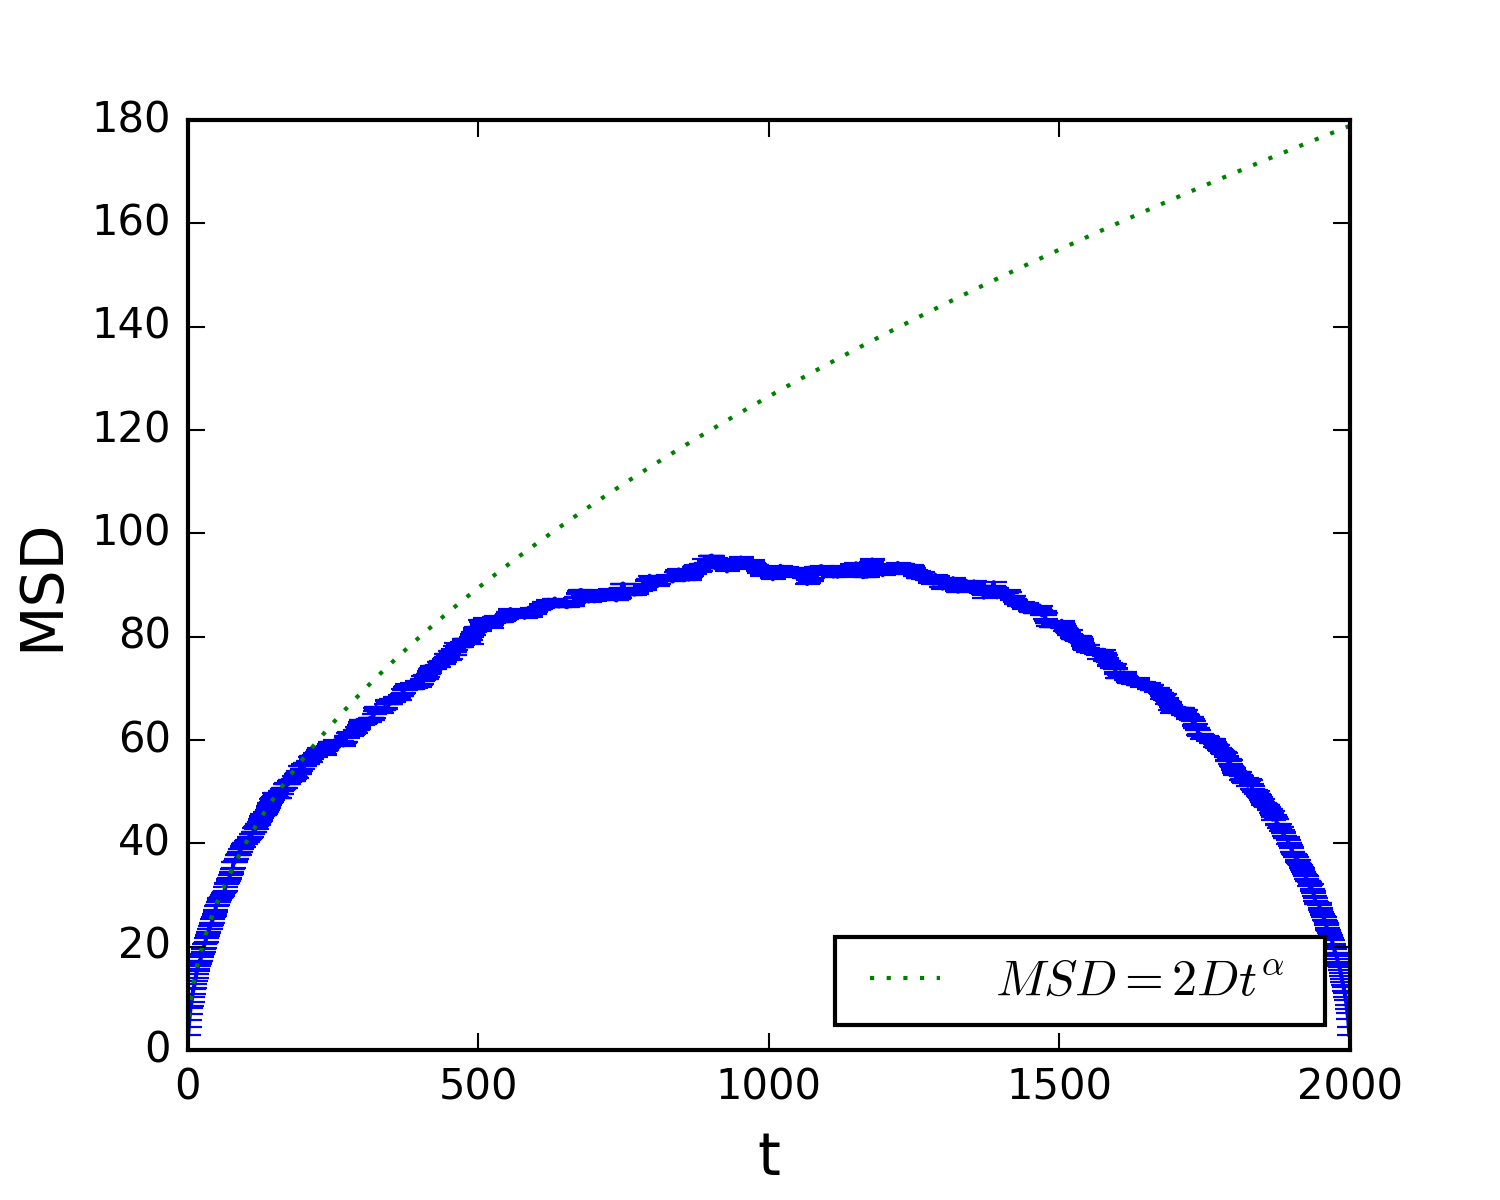
\includegraphics[width=0.5\textwidth]{./data/nocorrectionmsd.png}
  \label{fig:6}}
  \subfigure[Ensemble MSD with correction introduced in \cref{correction}. The side of the red bar indicates the threshold for the remaining increments for $M=2n$]{
  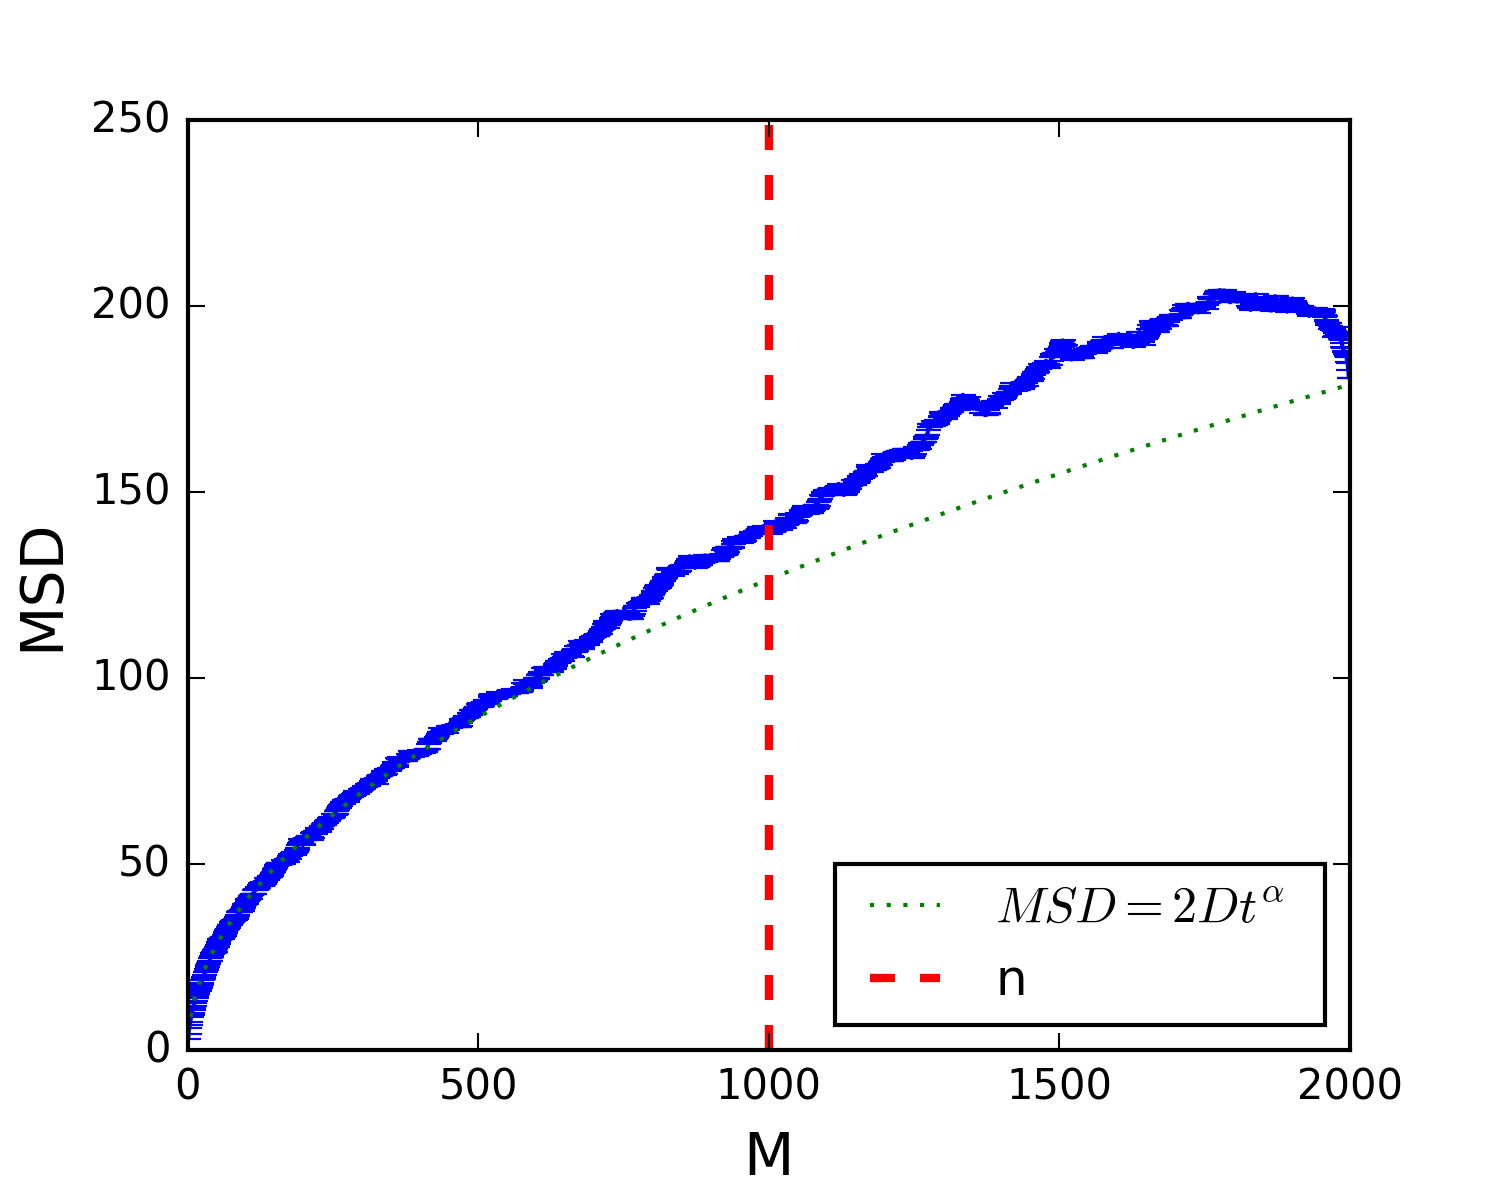
\includegraphics[width=0.5\textwidth]{./data/withcorrection_nocutoff.png}
  \label{fig:5}}
\end{figure}
This equation would be correct if we assumed fractional Brownian motion to be a Markovian process, which certainly is not the cause. This is also the reason why M have been chosen to be bigger than n. The presumption is, that the impact of the approximation would be negligible with increasing distance to $\Delta R_{M}$ and negligible at $\Delta R_{n}$. The impact on the ensemble averaged MSD can be seen in \cref{fig:5}. This can be thought of as a finite-time correction.

 %\item Laut dem Davies Harte Algorithmus wird außerdem das n-te Inkrement im Frequenzraum %umgeändert:
 %\begin{align}
 %\eta_{fbr_{g=n}} =\sqrt{Re(Z_g 2 n)} \mathcal{N}(0,1) 
 %\end{align}
 % Noch nicht verstanden warum!!
 \item With the reverse Fourier transform the fractional Brownian noise increments in the time domain result in:
 \begin{align}
 \xi_{k}= \frac{1}{2n} \sum_{l=0}^{2n-1}  \tilde{\xi}_l e^{\frac{2 \pi i l k }{2n}} \Delta z
 \end{align}
Only $n$ increments are taken into account $\xi_{j}$ for $j=(0,1,..,n)$.
\end{enumerate}
The described algorithm can be performed for every Cartesian component of the three dimensional fractional Brownian motion. The Cartesian component are not correlated.
\subsubsection{Lowen}
The previous algorithm had down draws in terms of convergence close to 0 and close to the overall simulation time. These problems are no longer present in the algorithm of Steven B. Lowen \cite{Lowen1999}. Lowens algorithm is both fast $(\mathcal{O}(NlogN))$ and exact. The algorithm goes as follows:
\begin{enumerate}
 \item Compute a periodic auto-covariance function of $R_{\xi}(n)$ of a stochastic process $\xi(n)$:
 \begin{align}
  R_{\xi}(n)=
  \begin{cases}
   \frac{1}{2}\left[1-\left(\frac{n}{N}\right)^{\alpha} \right]  & \text{ for    } 0 \leq n \leq N \\
   R_{\xi}(2N-n)  & \text{ for    } N \leq n \leq 2N 
  \end{cases}
 \end{align}
 \item Transform the auto-covariance function via FFT. The result is called the spectral density of the stochastic process $\xi(n)$:
  \begin{align}
   S_{\xi}(k)= FFT(R_{\xi}(n))
  \end{align}
 \item Calculate $\tilde\xi(k)$ the Fourier transform of the stochastic process $\xi(n)$:
 \begin{align}
  \tilde\xi(k)=
  \begin{cases}
     0  & \text{ for    } k=0 \\    
     exp(i \theta) \eta \sqrt{S_{\xi}(k)}  & \text{ for    } 0 \leq k \leq N \\
     \eta \sqrt{S_{\xi}(k)}  & \text{ for    } k = N \\
     \tilde\xi^{*}(2N-k) & \text{ for    } N \leq k \leq 2N 
  \end{cases}
 \end{align}
 $\tilde\xi^{*}$ denotes the complex conjugate of $\tilde\xi$. $\theta$ is a random variable uniformly distributed  in $(0,2\pi]$. $\eta$ is a random Gaussian variable with zero mean and variance 1 ($\mathcal{N}(0,1)$).  
 \item Perform the inverse Fourier transform on $\tilde\xi(k)$ and use the first half of the resulting stochastic process $\xi(n)$ multiplied by a factor:
 \begin{align}
  \xi(n)&=FFT^{-1}(\tilde\xi(k)) \\
  B^{\alpha}_n&=  \sqrt{2 K_{\alpha} N^{\alpha} \Delta t^{\alpha}} (\xi(n)- \xi(0)) \qquad \qquad \qquad \text{for    } 0 \leq n \leq N
 \end{align}
\end{enumerate}
Lets check the resulting auto-covariance function. 
\begin{align}
  & Cov[B^{\alpha}_n,B^{\alpha}_m]= 2 K_{\alpha} \Delta t^{\alpha} N^{\alpha} \langle (\xi(n)- \xi(0)) ((\xi(m)- \xi(0))\rangle \\
 &=  2 K_{\alpha} \Delta t^{\alpha} N^{\alpha}\langle\xi(n)\xi(m)\rangle -\langle \xi(0) \xi(m)\rangle - \langle \xi(0) \xi(n)\rangle +\langle \xi(0)^2\rangle \\ 
 &=\frac{2 K_{\alpha} \Delta t^{\alpha}}{2}[n^{\alpha}-2(m-n)^{\alpha}+n^{\alpha}]\qquad \qquad \qquad \qquad  \text{ for }  n < m
\end{align}
The auto-covariance function indeed satisfies the condition for fBm with variance similar to \cref{diffusionvariance}. In step 3 the phase and amplitude of the Fourier transform  $\xi(m)$ were chosen to be random  as suggested in \cite{Timmer1995}. The second derivative of $R_{\xi}(n) $ is positive. $R_{\xi}(n) $ results in a periodic function with non negative curvature. Its Fourier transform $S_{\xi}(k)$ is , real, symmetric  and non-negative for all k. $S_{\xi}(k)$ is then a valid power spectral density function of the discrete-time periodic process $\xi(n)$ with period $2n$ and  $R_{\xi}(n)$ its valid auto-covariance function \cite{Lowen1999}. This algorithm is actually using the property of Brownian scaling \cref{Brownianscaling} to generate a realization of fBm  with non negative auto-covariance function. The algorithm was implemented in c++ with a 1 dimension Fast Fourier transform from the package FFTW3. FFTW computes an unnormalized DFT. Thus, computing a forward followed by a backward transform results in the original array scaled by the size of the array. The size of the array is $2N$  in Lowens algorithm. Thus a random variable should be divided by $\sqrt{2N}$ to have a normalized FFT.

\subsubsection{Testing of the Algorithm}
\begin{figure}[h!]
\centering
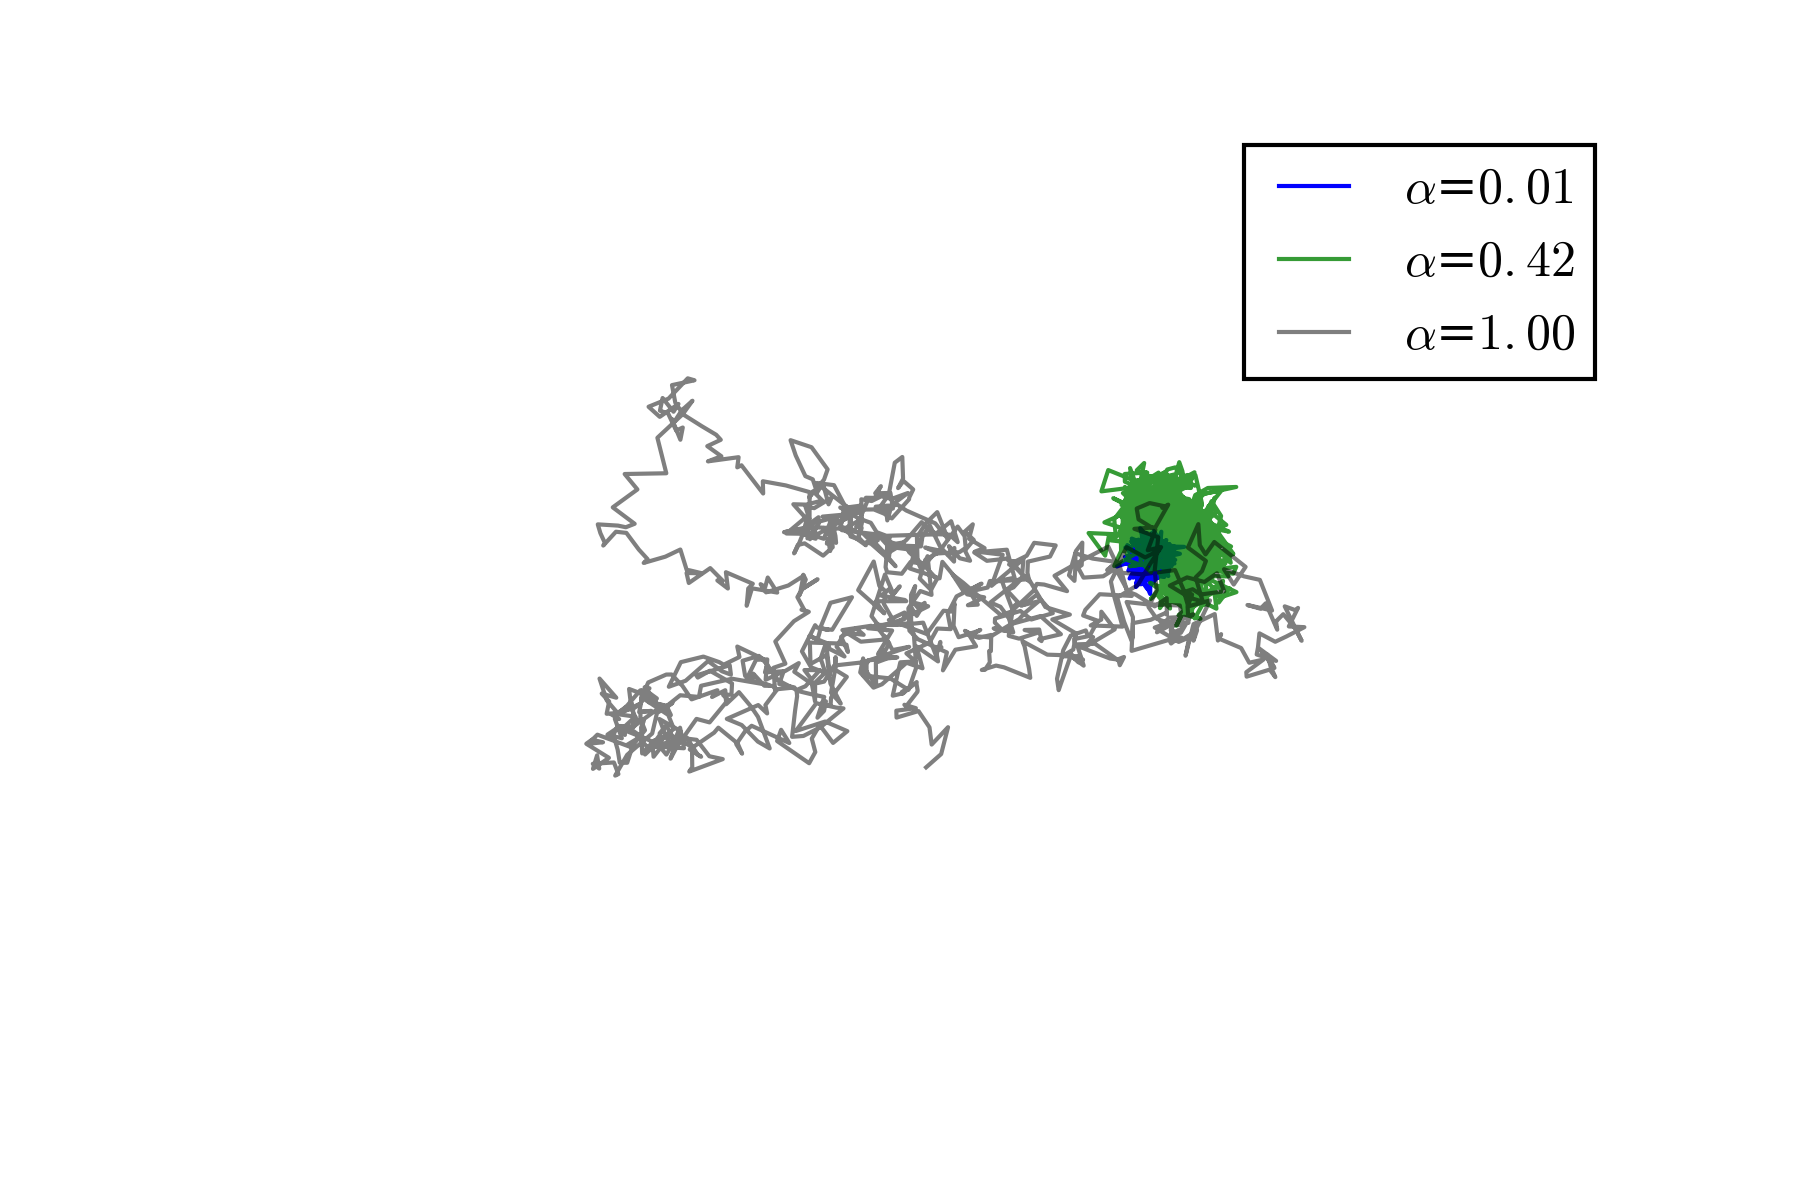
\includegraphics[width=\textwidth]{./data/trajectories_differentalpha.png}
\caption{shows 3D trajectories for different $\alpha$ generated with the Lowen algorithm for $K_{\alpha}=1$, $\Delta t=1$ and the trajectory length $M=1000$.}
\label{alphachangetrajectory}
\end{figure}
The algorithms were implemented in python and c++. For the c++ implementation a wrapper to python was added. All algorithms have been analyzed by an analysis class. The c++ implementation is using FFTW library for the Fast Fourier Transform and Mersenne-Twister (gsl\texttt{\textunderscore}rng\texttt{\textunderscore}mt19937) as the random number generator. The python implementation was developed beforehand and  only serves as a reference. Python uses the numpy.fft library for the Fast Fourier Transform and also the Mersenne-Twister random number generator.\newline
To get insight into stochastic algorithms observables have to by studied. They are generally averaged values. The algorithm was designed to produce fBm. The most important quantity to analyze is the  MSD. It can be calculated as the ensemble-, time- or time-ensemble-average. A comparison between the average types are plotted in \cref{fig:4} .A difference in time and ensemble averages would show a violation of ergodicity. The tails of the time and ensemble-time averages are increasingly deviate from the theoretical values for long lag times due to decreasing statistics. In the following figures all MSD plots are ensemble averages. They are computationally cheaper. It can be  seen, that  tends to result in  too MSDs for small lag times. This is caused by the finite amount of samples in the discrete Fourier transform until know reducing these effects is only possible by reducing the time step.
Another MSD influencing variable is the anomalous coefficient $\alpha$. The influence on the MSD is shown in \cref{alphachange} . In the limit of Brownian motion $\alpha=1$ the artifacts for small lag-times vanish. The downside are longer simulation times for the same time in the simulation.
\begin{comment}
 

\begin{figure}[h!]
  \centering
  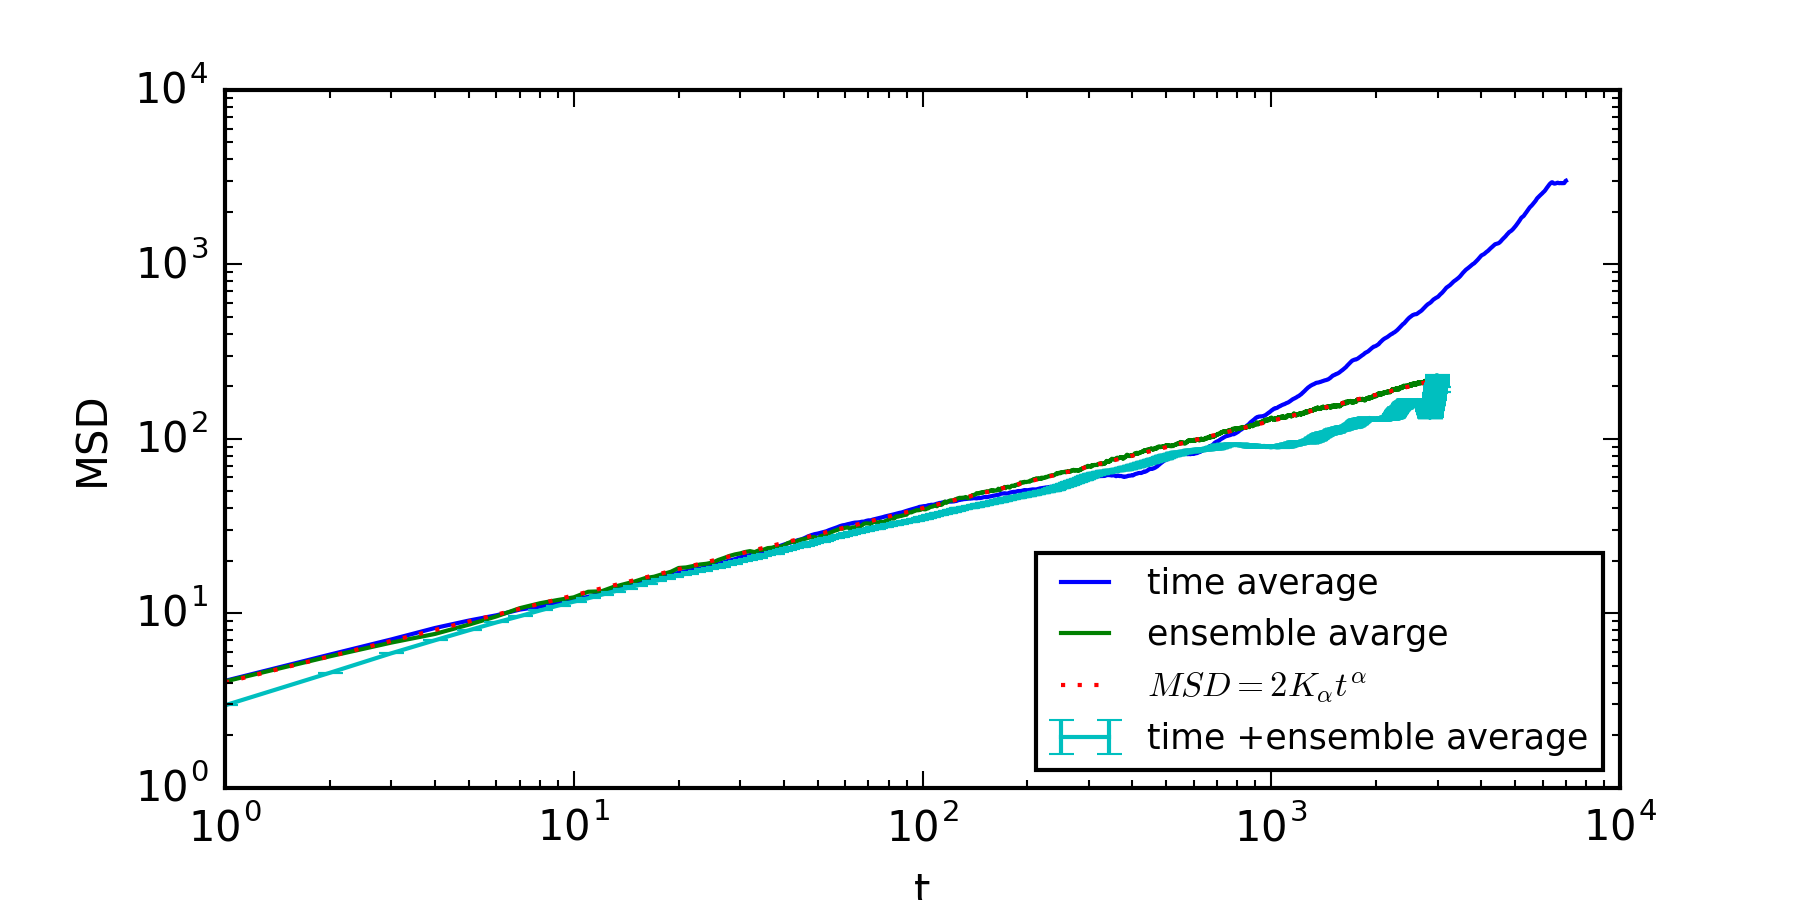
\includegraphics[width=\textwidth]{./data/averages_comparison.png}
  \captionsetup{width=\linewidth}
  \captionof{figure}{Comparison of Mean-Square-Displacements between time-average, ensemble-average and time-ensemble-average for $D=2$, $\alpha=0.5$, $\Delta t=1$. For the time ensemble average only 10 trajectories have been taken.}
  \label{fig:4}
\end{figure}
\newline \noindent The influence of the time step size is shown in \cref{fig:3} . The deviation from the expected value is linearly dependent on the amount of samples in the interval.
\begin{figure}[h!]
  \centering
  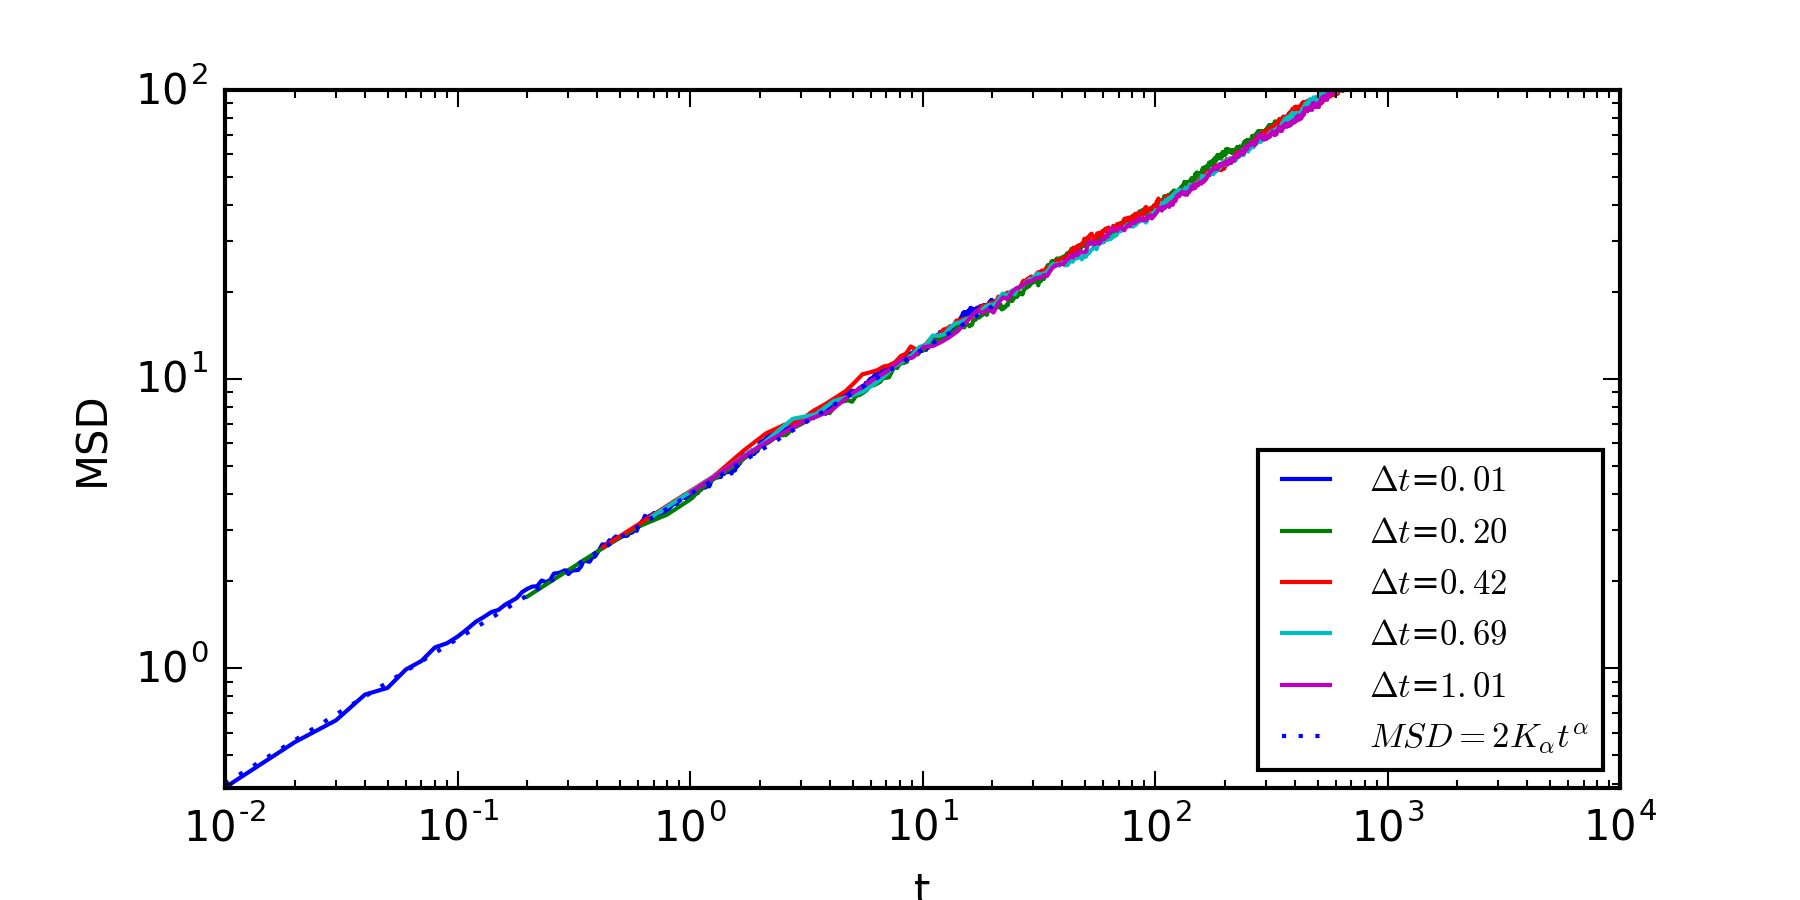
\includegraphics[width=\textwidth]{./data/dt_change.png}
  \captionsetup{width=\linewidth}
  \captionof{figure}{Comparison of ensemble averaged Mean-Square-Displacements with different $\Delta t$ for $D=2$, $\alpha=0.5$. }
  \label{fig:3}
\end{figure} 
\noindent 
\begin{figure}[h!]
\centering
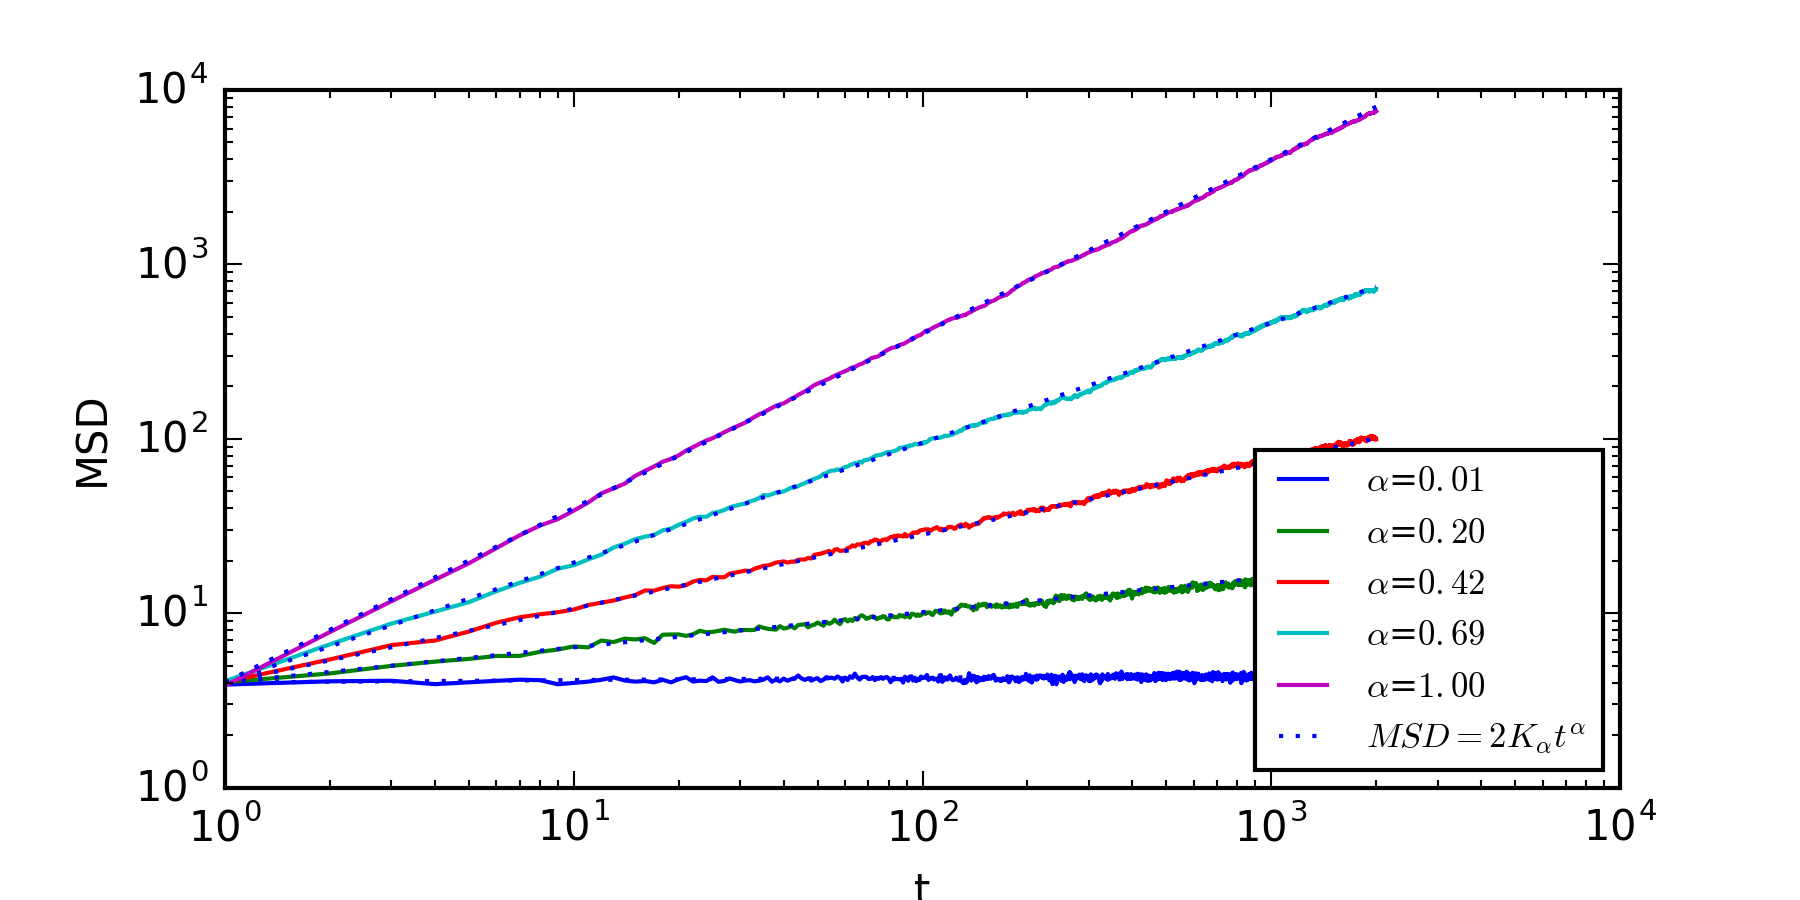
\includegraphics[width=\textwidth]{./data/alpha_change.png}
\caption{Ensemble averaged MSD for different $\alpha$  with $K_{\alpha}=2$ , $N=2000$, $n=2000$ , $\Delta t = 1$, $M=2n$.}
\label{alphachange}
\end{figure}
\begin{figure}[h!]
\centering
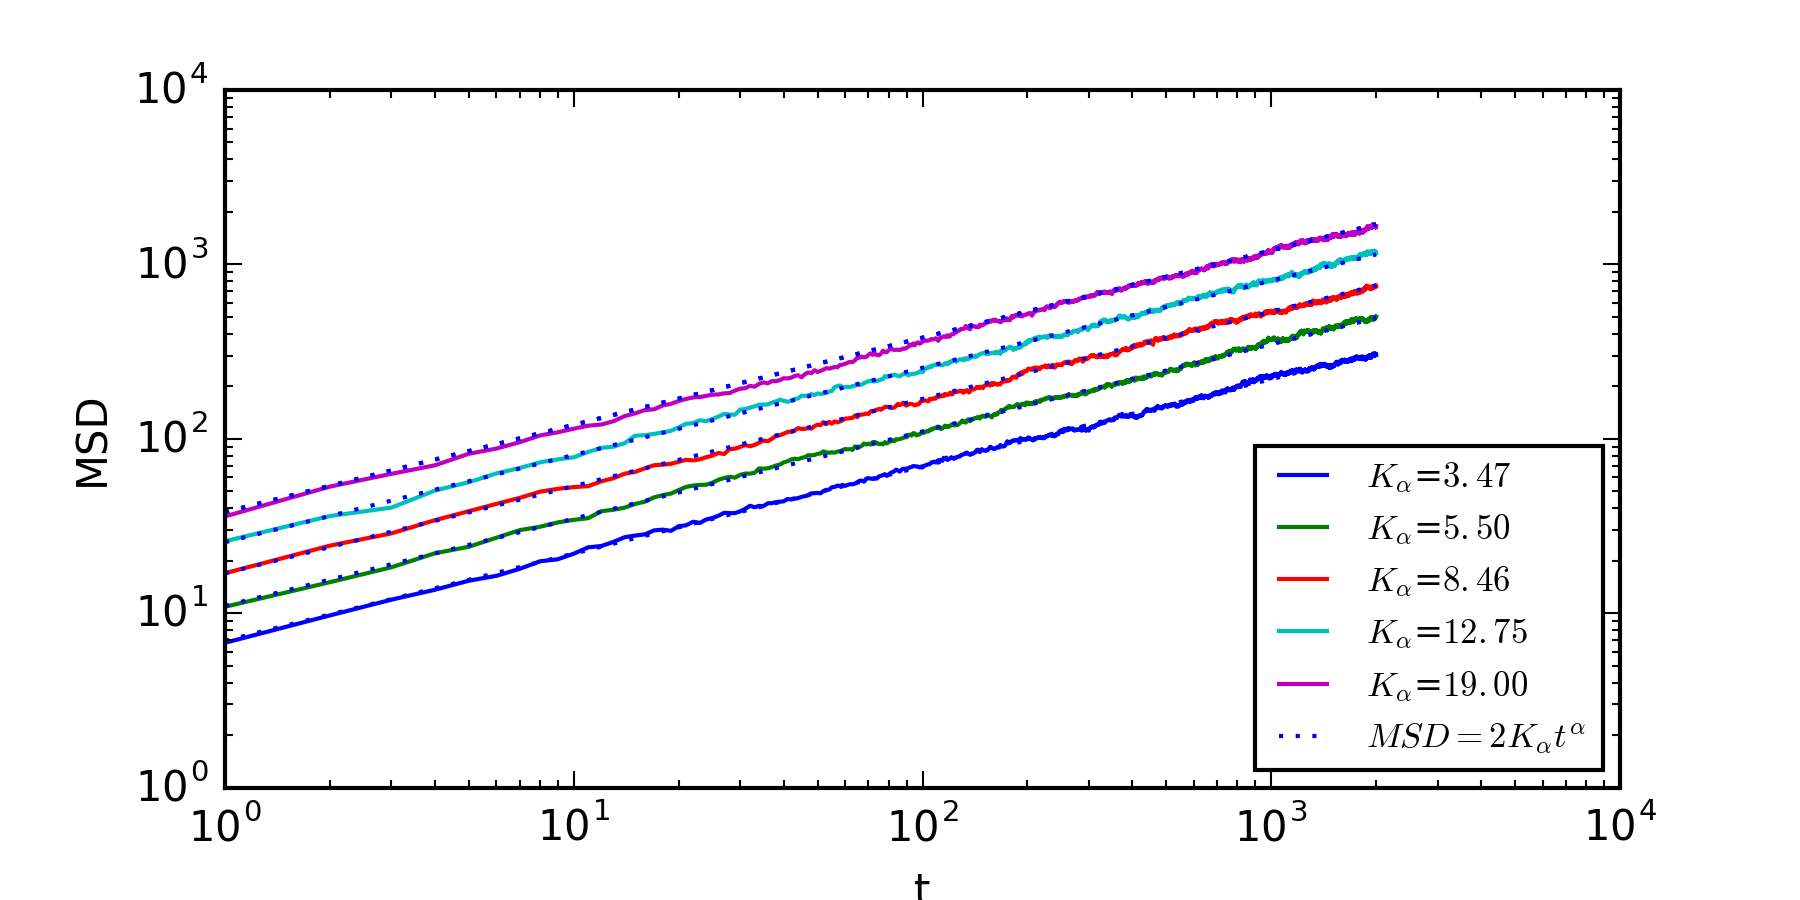
\includegraphics[width=\textwidth]{./data/K_alpha_change.png}
\caption{Ensemble averaged MSD for different $K_\alpha$. with $\alpha=0.5$ , $N=2000$, $n=2000$ , $\Delta t = 1$, $M=2n$.}
\label{kalphachange}
\end{figure}
\noindent The generalized diffusion coefficient has also bin varied. The influence on the MSD can be seen in \cref{kalphachange} . The change of $K_{alpha}$ is not influencing the quality of the simulation.
\begin{figure}[h!]
\begin{minipage}{\textwidth}
\centering
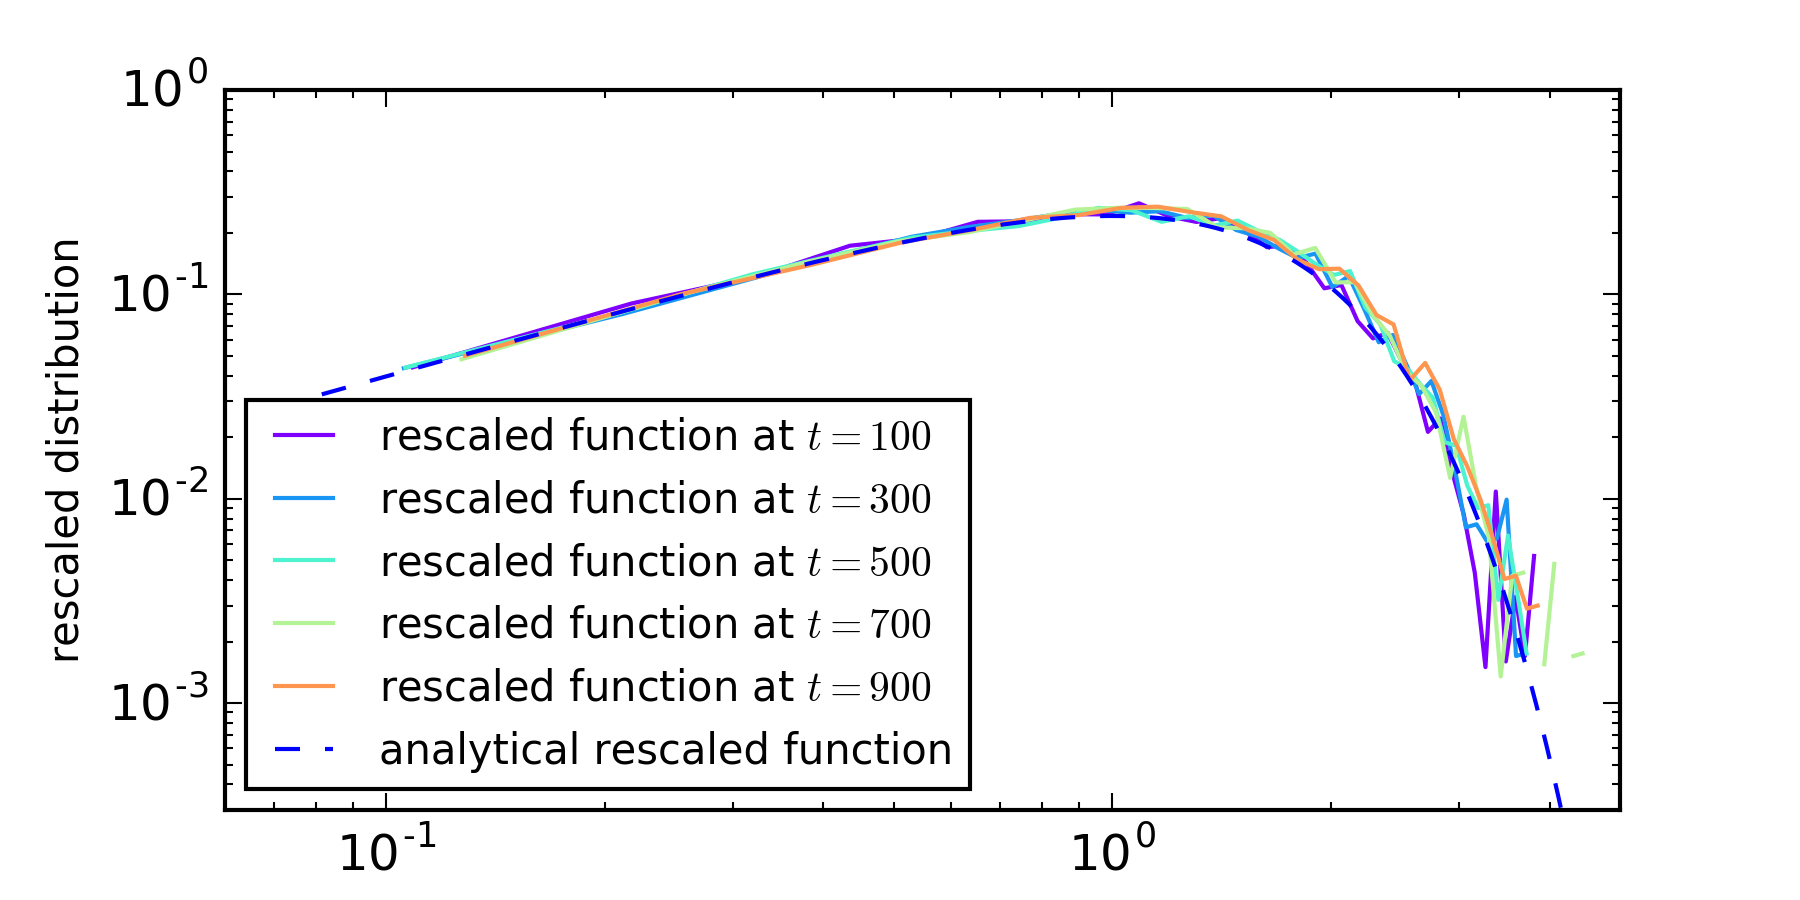
\includegraphics[width=\textwidth]{./data/rescaled.png}
\caption{The scale free form of the Propagator at different times as introduced in \cref{scalefreeformfrac}. With $K_{\alpha}=2$, $\alpha=0.5 $, $N=10000$ , $\Delta t = 1$, $M=2n$.  }
\label{rescaledfigure}
\end{minipage}
\begin{minipage}{\textwidth}
\centering
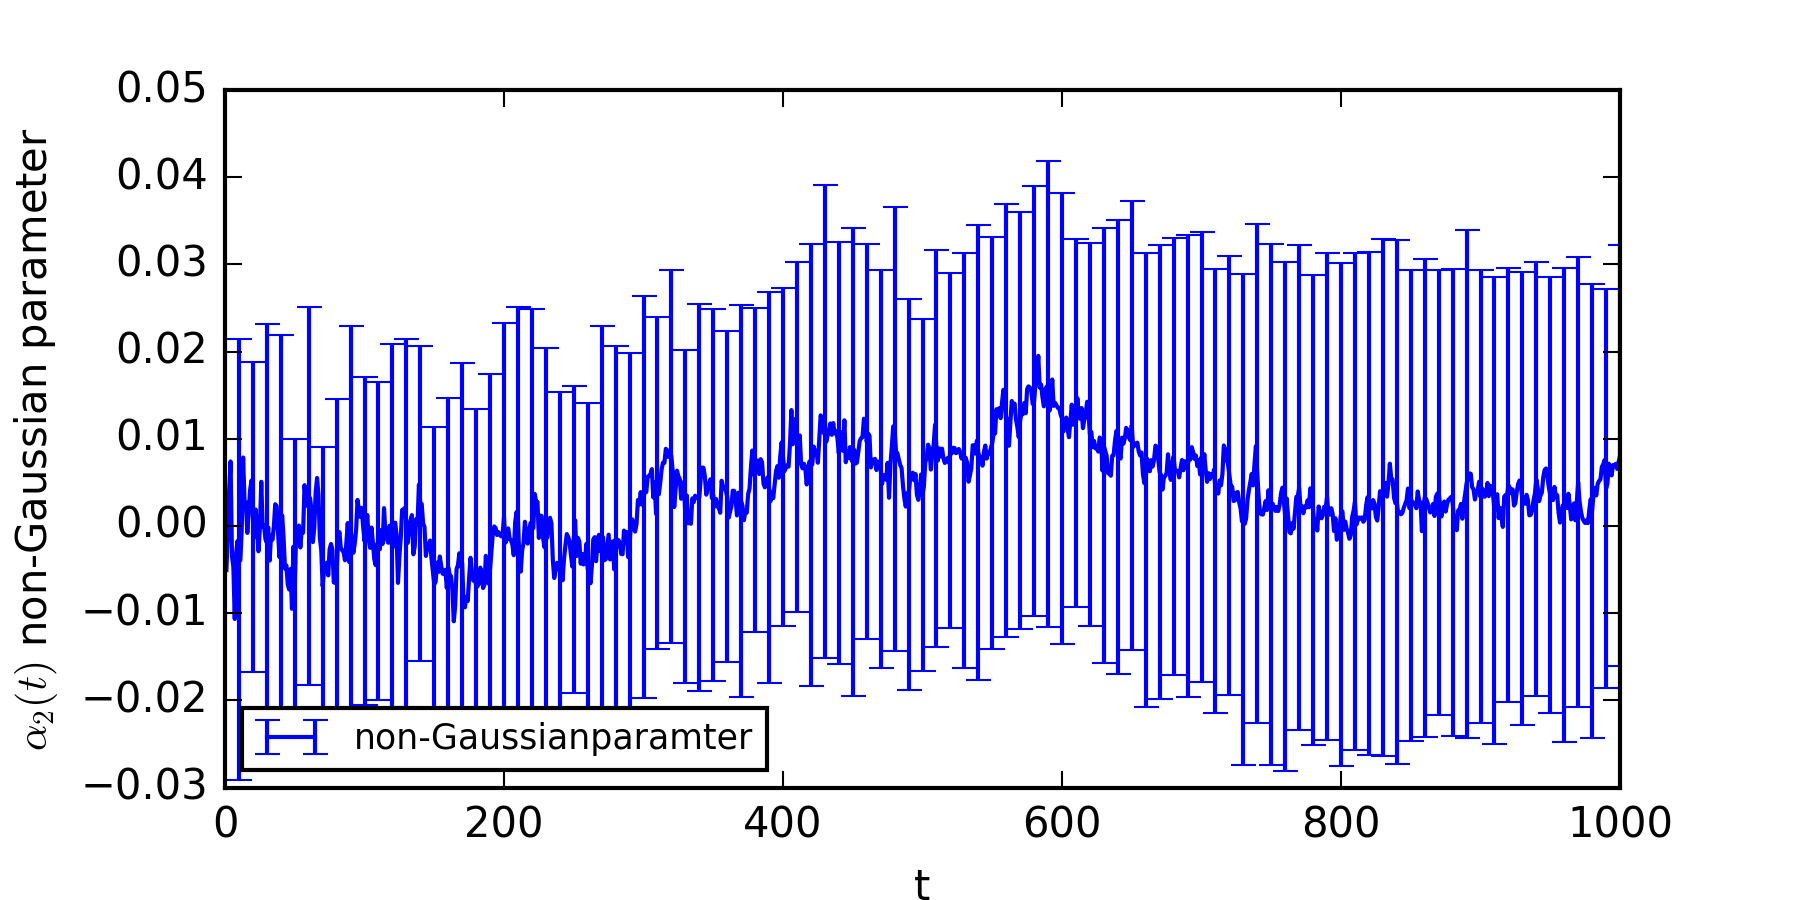
\includegraphics[width=\textwidth]{./data/nongaussian.png}
\caption{Non-Gaussian-Parameter (as introduced in \cref{nongaussian2}) With $K_{\alpha}=2$ , $N=5000$, $n=1001$ , $\Delta t = 1$, $M=2n$ averaged over $30$ non-Gaussian-Parameter with its variance displayed as an error bar.}
 \centering
\end{minipage}
\end{figure}

\begin{figure}[h!]
\centering
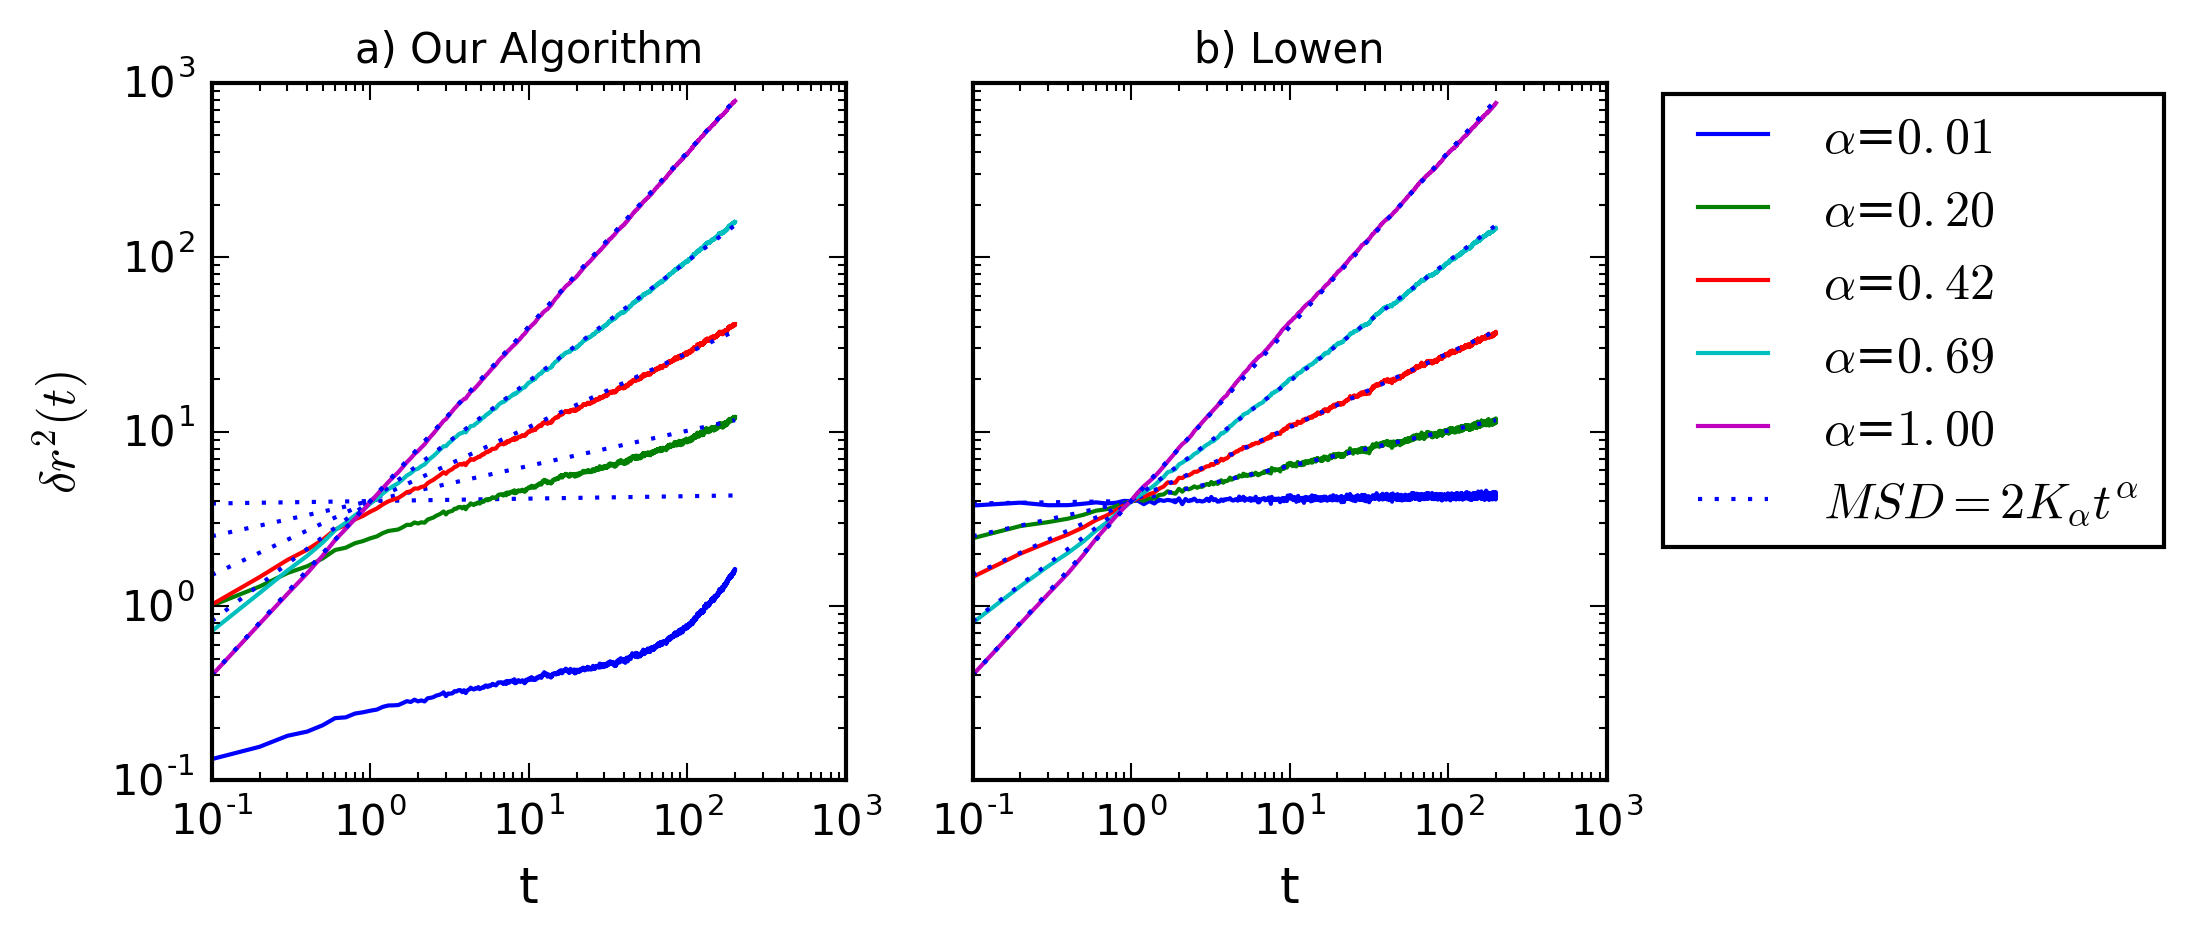
\includegraphics[width=\textwidth]{./data/alpha_changeboth.png}
\caption{Both Plots show an ensemble average MSD over $N=2000$ trajectories for $0.1<\alpha<1.0$  with $K_{\alpha}=2$ , $M=2000$ , $\Delta t = 0.1$, with a) Our algorithm and b) Lowen algorithm.}
\label{alphachange}
\end{figure}
\noindent As a property of self similarity a scale free version of the density distribution can be calculated \cref{sectionfrac} \cref{scalefreeformfrac}. The scale free density distribution is not depended on time but overlaps for all times. The algorithm is performing as predicted and computing a self-similar process. The scale free distribution is extracted from the simulation for different times and compared to the analytical result. The graph can be seen in \cref{rescaledfigure}.  

 
\end{comment}


\begin{figure}[h!]
\centering
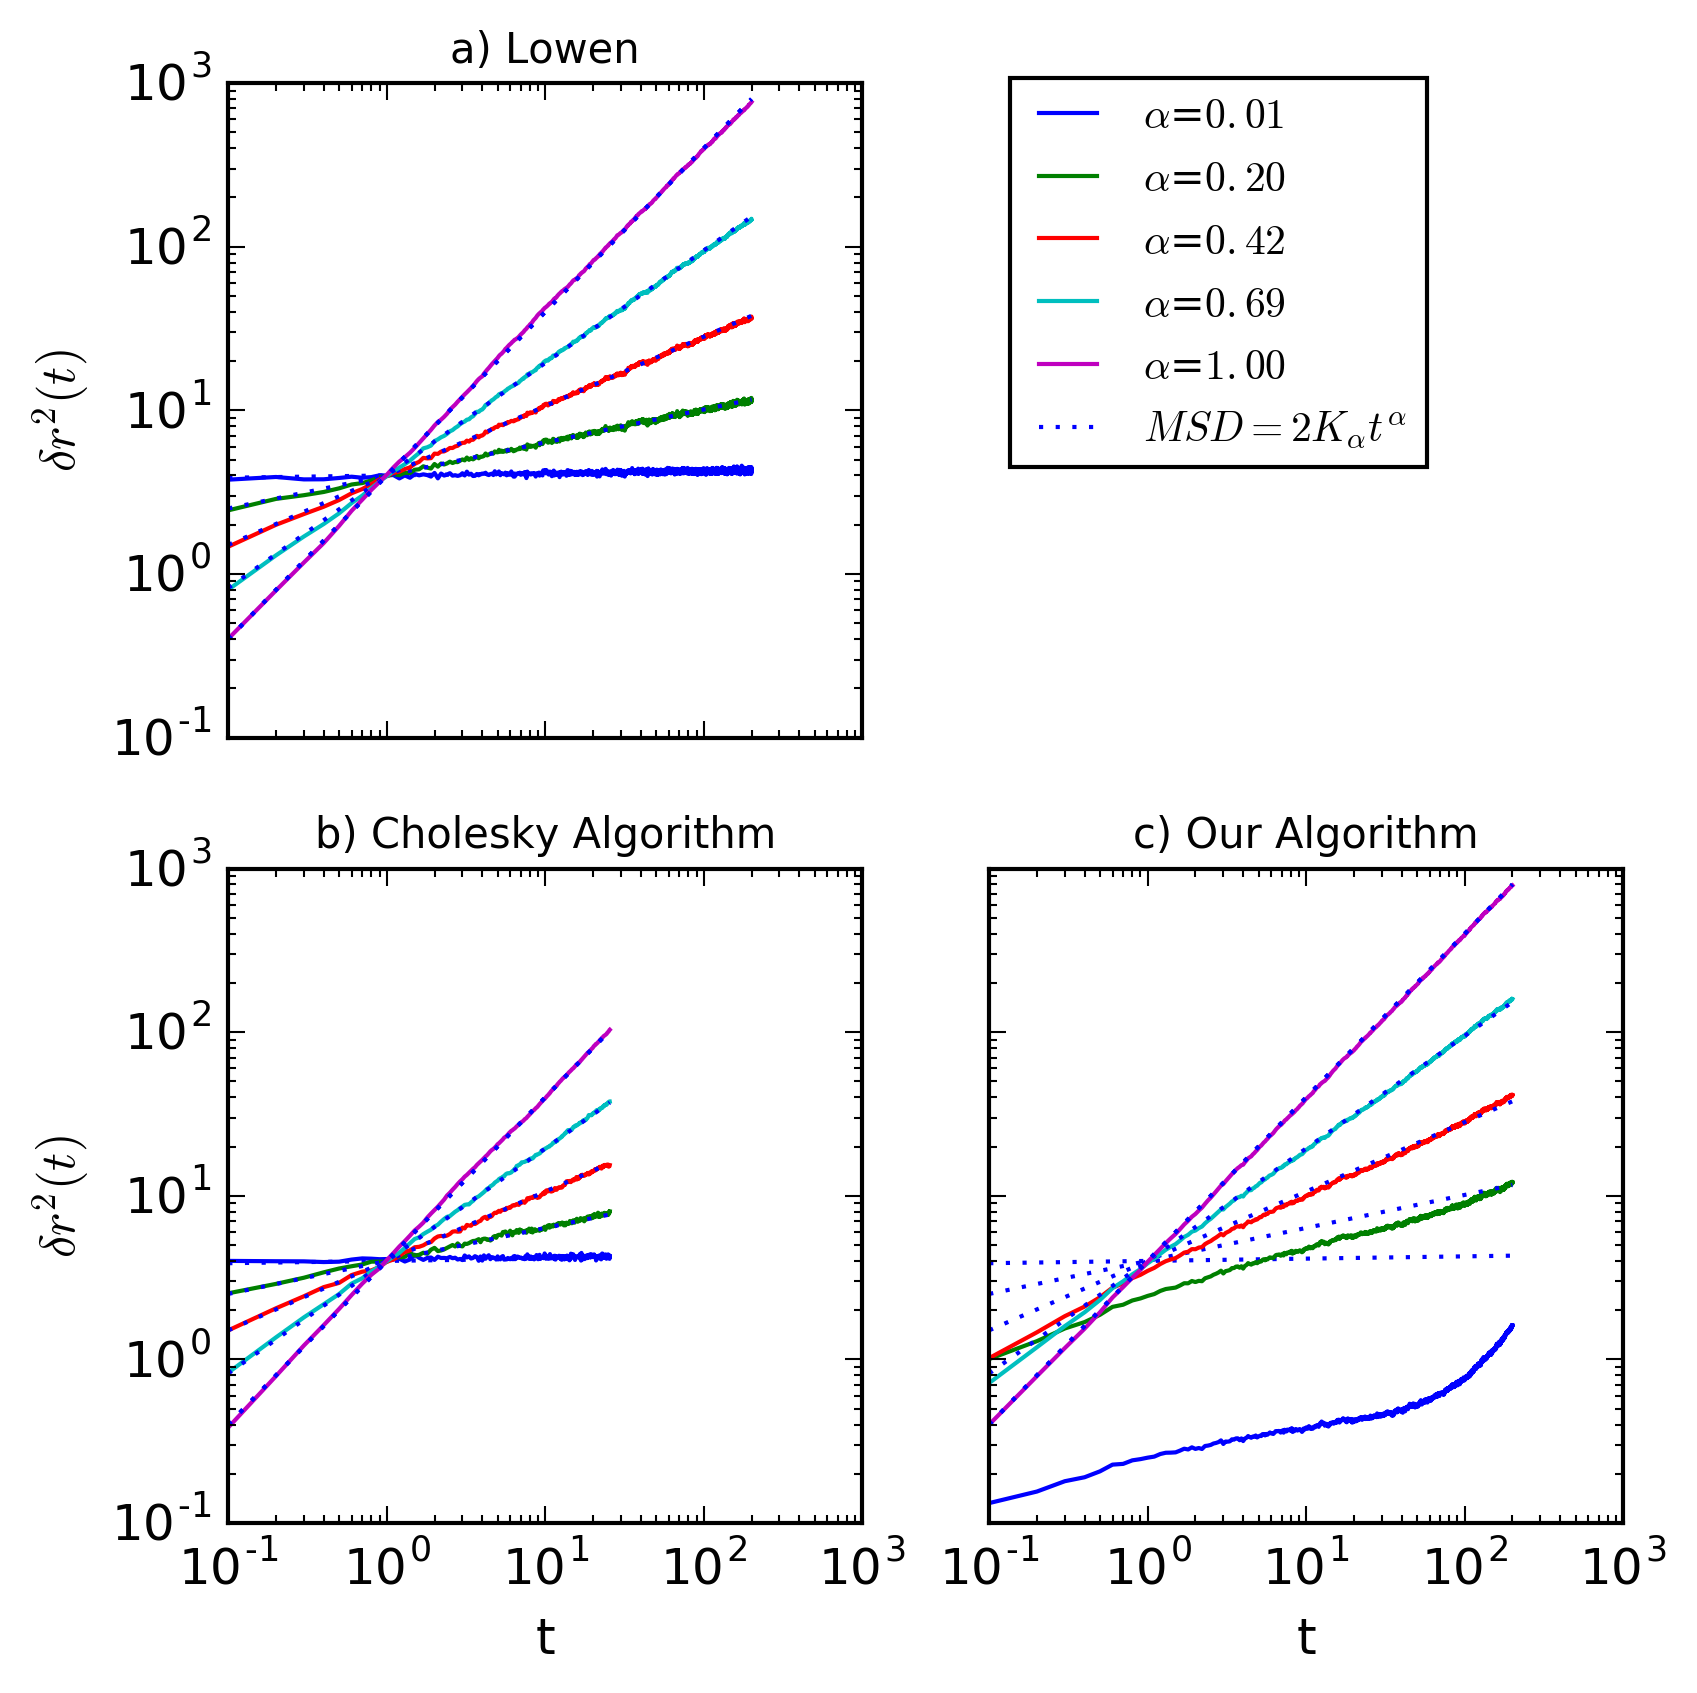
\includegraphics[width=\textwidth]{./data/alpha_changethree.png}
\caption{All three plots show an ensemble averaged MSD over $N=2000$ trajectories for $0.1<\alpha<1.0$  with $K_{\alpha}=2$ ,$\Delta t = 0.1$ and trajectory length $M=2000$  for Our and Lowen algorithm, $M=256$ for Choleski algorithm. a) Our algorithm and b) Lowen algorithm c) Choleski algorithm.}
\label{alphachange}
\end{figure}

\begin{figure}[h!]
\centering
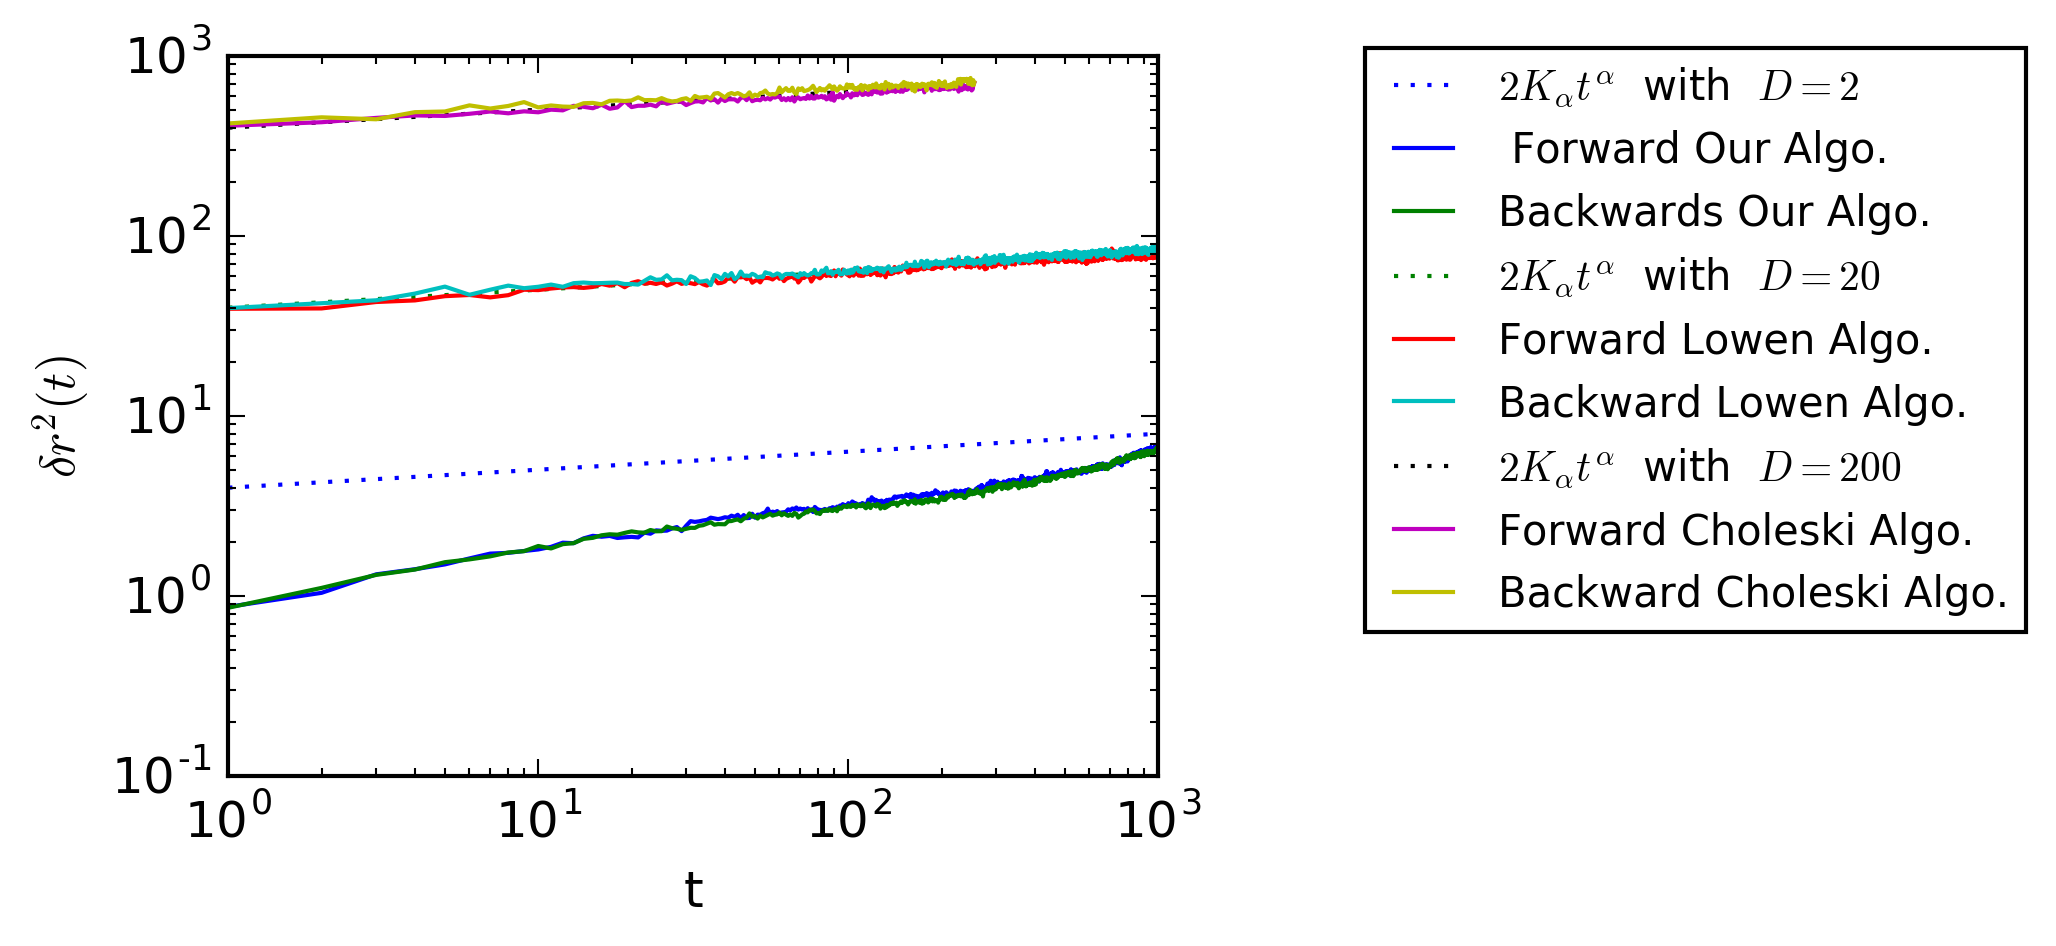
\includegraphics[width=\textwidth]{./data/changeintime.png}
\caption{The plot show ensemble averaged MSDs over $N=2000$ trajectories for $\alpha =0.1$, $\Delta t = 0.1$ and trajectory length $M=1000$ and $K_{\alpha}=2$ for Our algorithm, $M=1000$  $K_{\alpha}=20 $ for Lowen algorithm and  $M=256$  $K_{\alpha}=200$ for Choleski algorithm.}
\label{changeintime}
\end{figure}
\begin{figure}[h!]
\centering
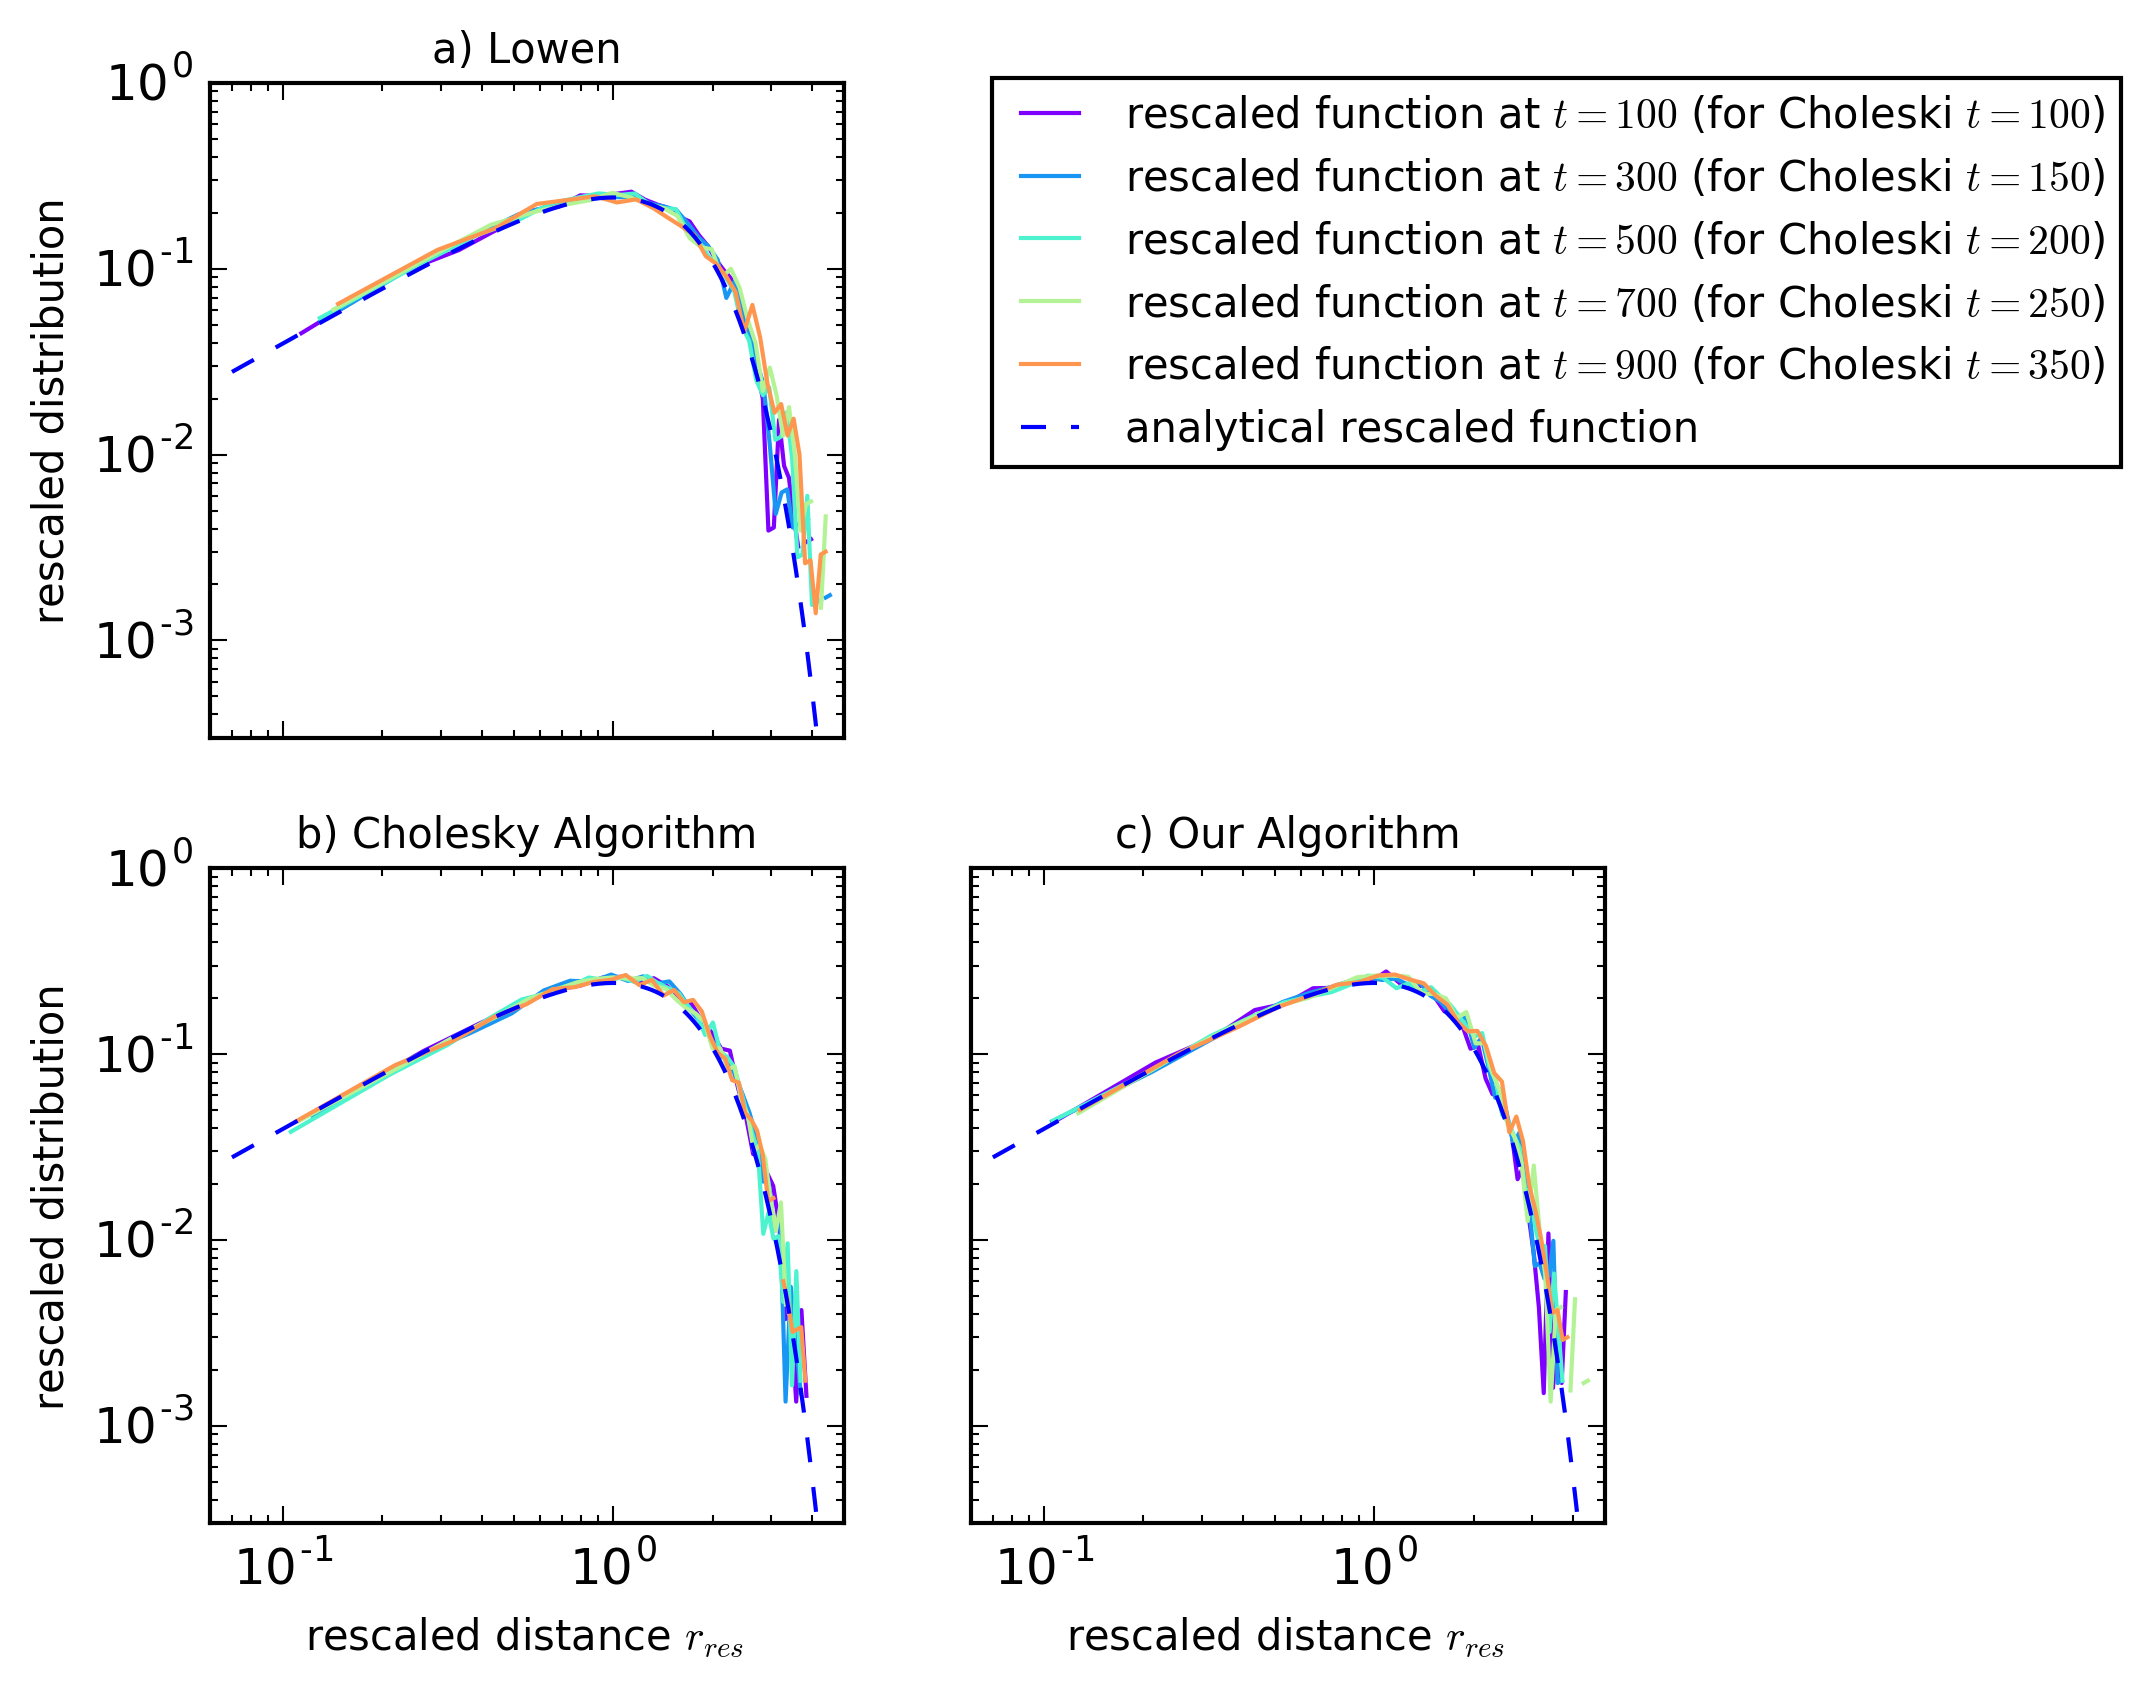
\includegraphics[width=\textwidth]{./data/scaledfunctionneu.png}
\caption{All three plots show the scale free form of the propagator at different times as introduced in \cref{scalefreeformfrac} as an histogram over $N=10000$ trajectories for $\alpha=0.5$  with $K_{\alpha}=2$ ,$\Delta t = 0.1$ for all three algorithm, at different times $100<t<900$}
\label{rescaledfunction}
\end{figure}

\noindent As a property of self similarity a scale free version of the density distribution can be calculated \cref{sectionfrac} \cref{scalefreeformfrac}. The scale free density distribution is not depended on time but overlaps for all times. The algorithm is performing as predicted and computing a self-similar process. The scale free distribution is extracted from the simulation for different times and compared to the analytical result. The graph can be seen in \cref{rescaledfigure}.  

\begin{figure}[h!]
\centering
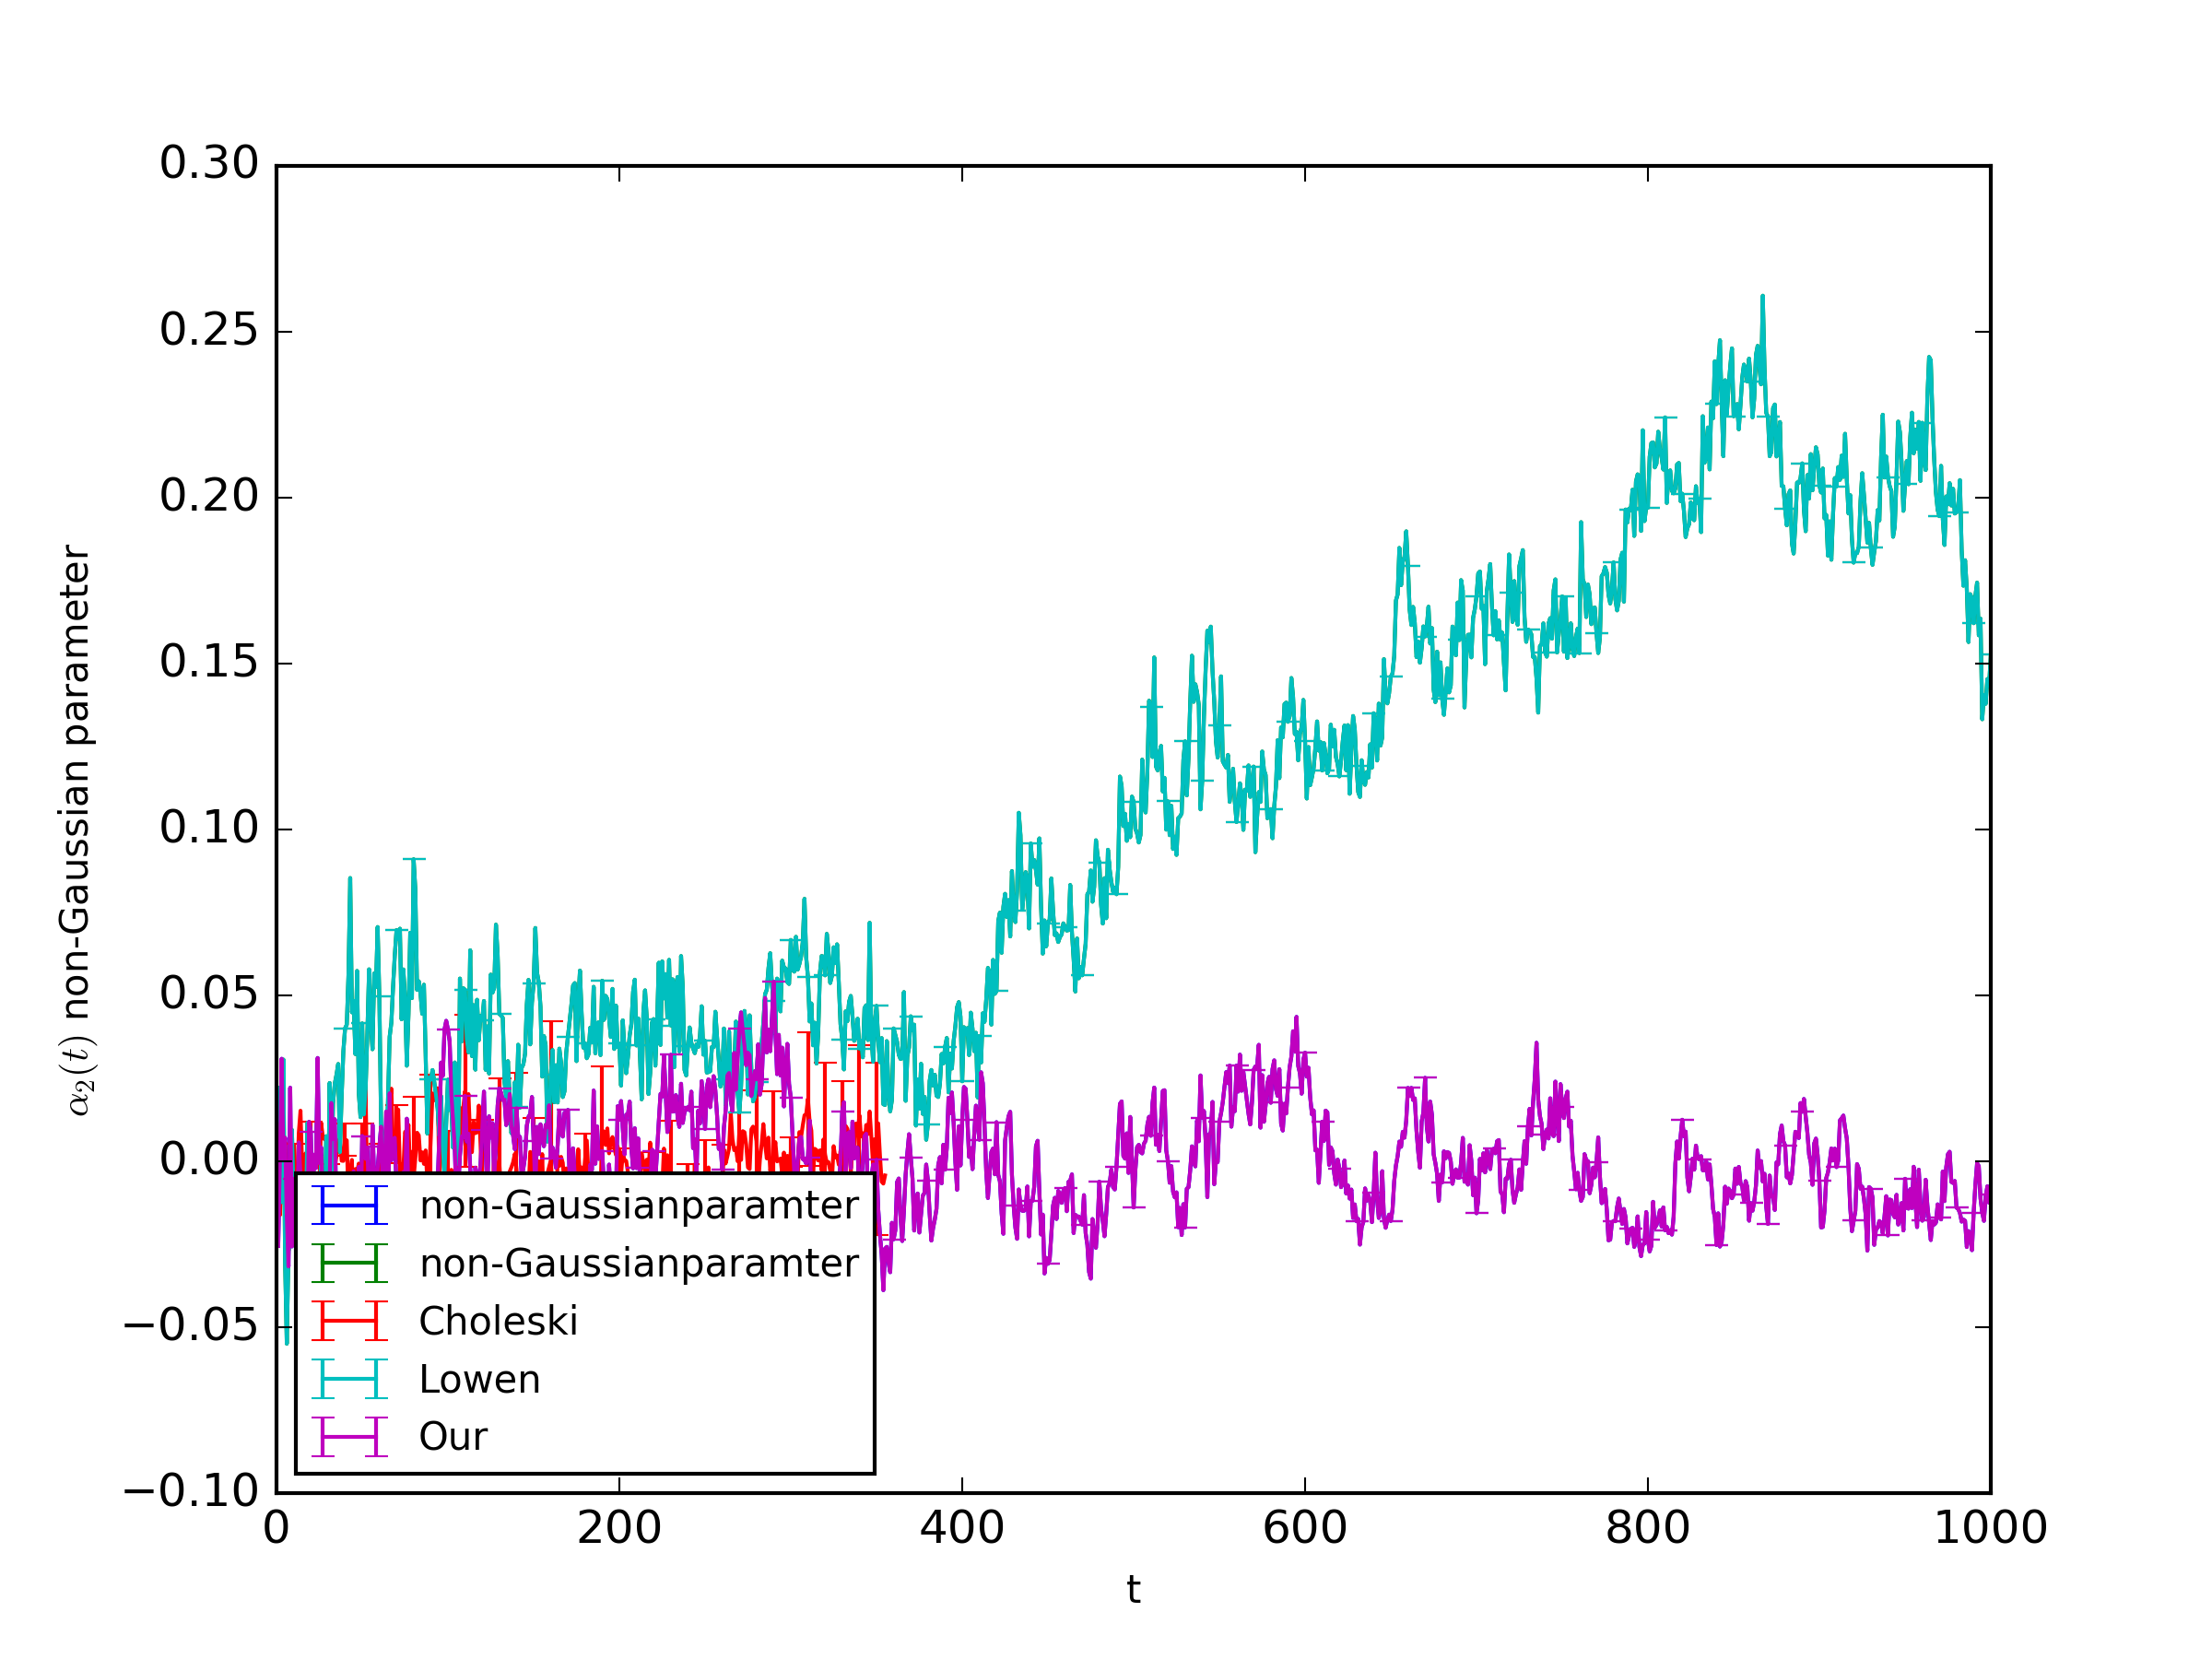
\includegraphics[width=\textwidth]{./data/nongaussianneu.png}
\caption{Non-Gaussian-Parameter as introduced in \cref{nongaussian2} for all three algorithms with $K_{\alpha}=2$ , $N=5000$, (Lowen and Our $M=1001$; Choleski $M=356$), $\Delta t = 1$  averaged over $50$ non-Gaussian-Parameter with its variance displayed as an error bar.}}
\label{nongaussian}
\end{figure}

\noindent As a property of self similarity a scale free version of the density distribution can be calculated \cref{sectionfrac} \cref{scalefreeformfrac}. The scale free density distribution is not depended on time but overlaps for all times. The algorithm is performing as predicted and computing a self-similar process. The scale free distribution is extracted from the simulation for different times and compared to the analytical result. The graph can be seen in \cref{rescaledfigure}.  
\begin{comment}

\begin{figure}[h]
  \centering
  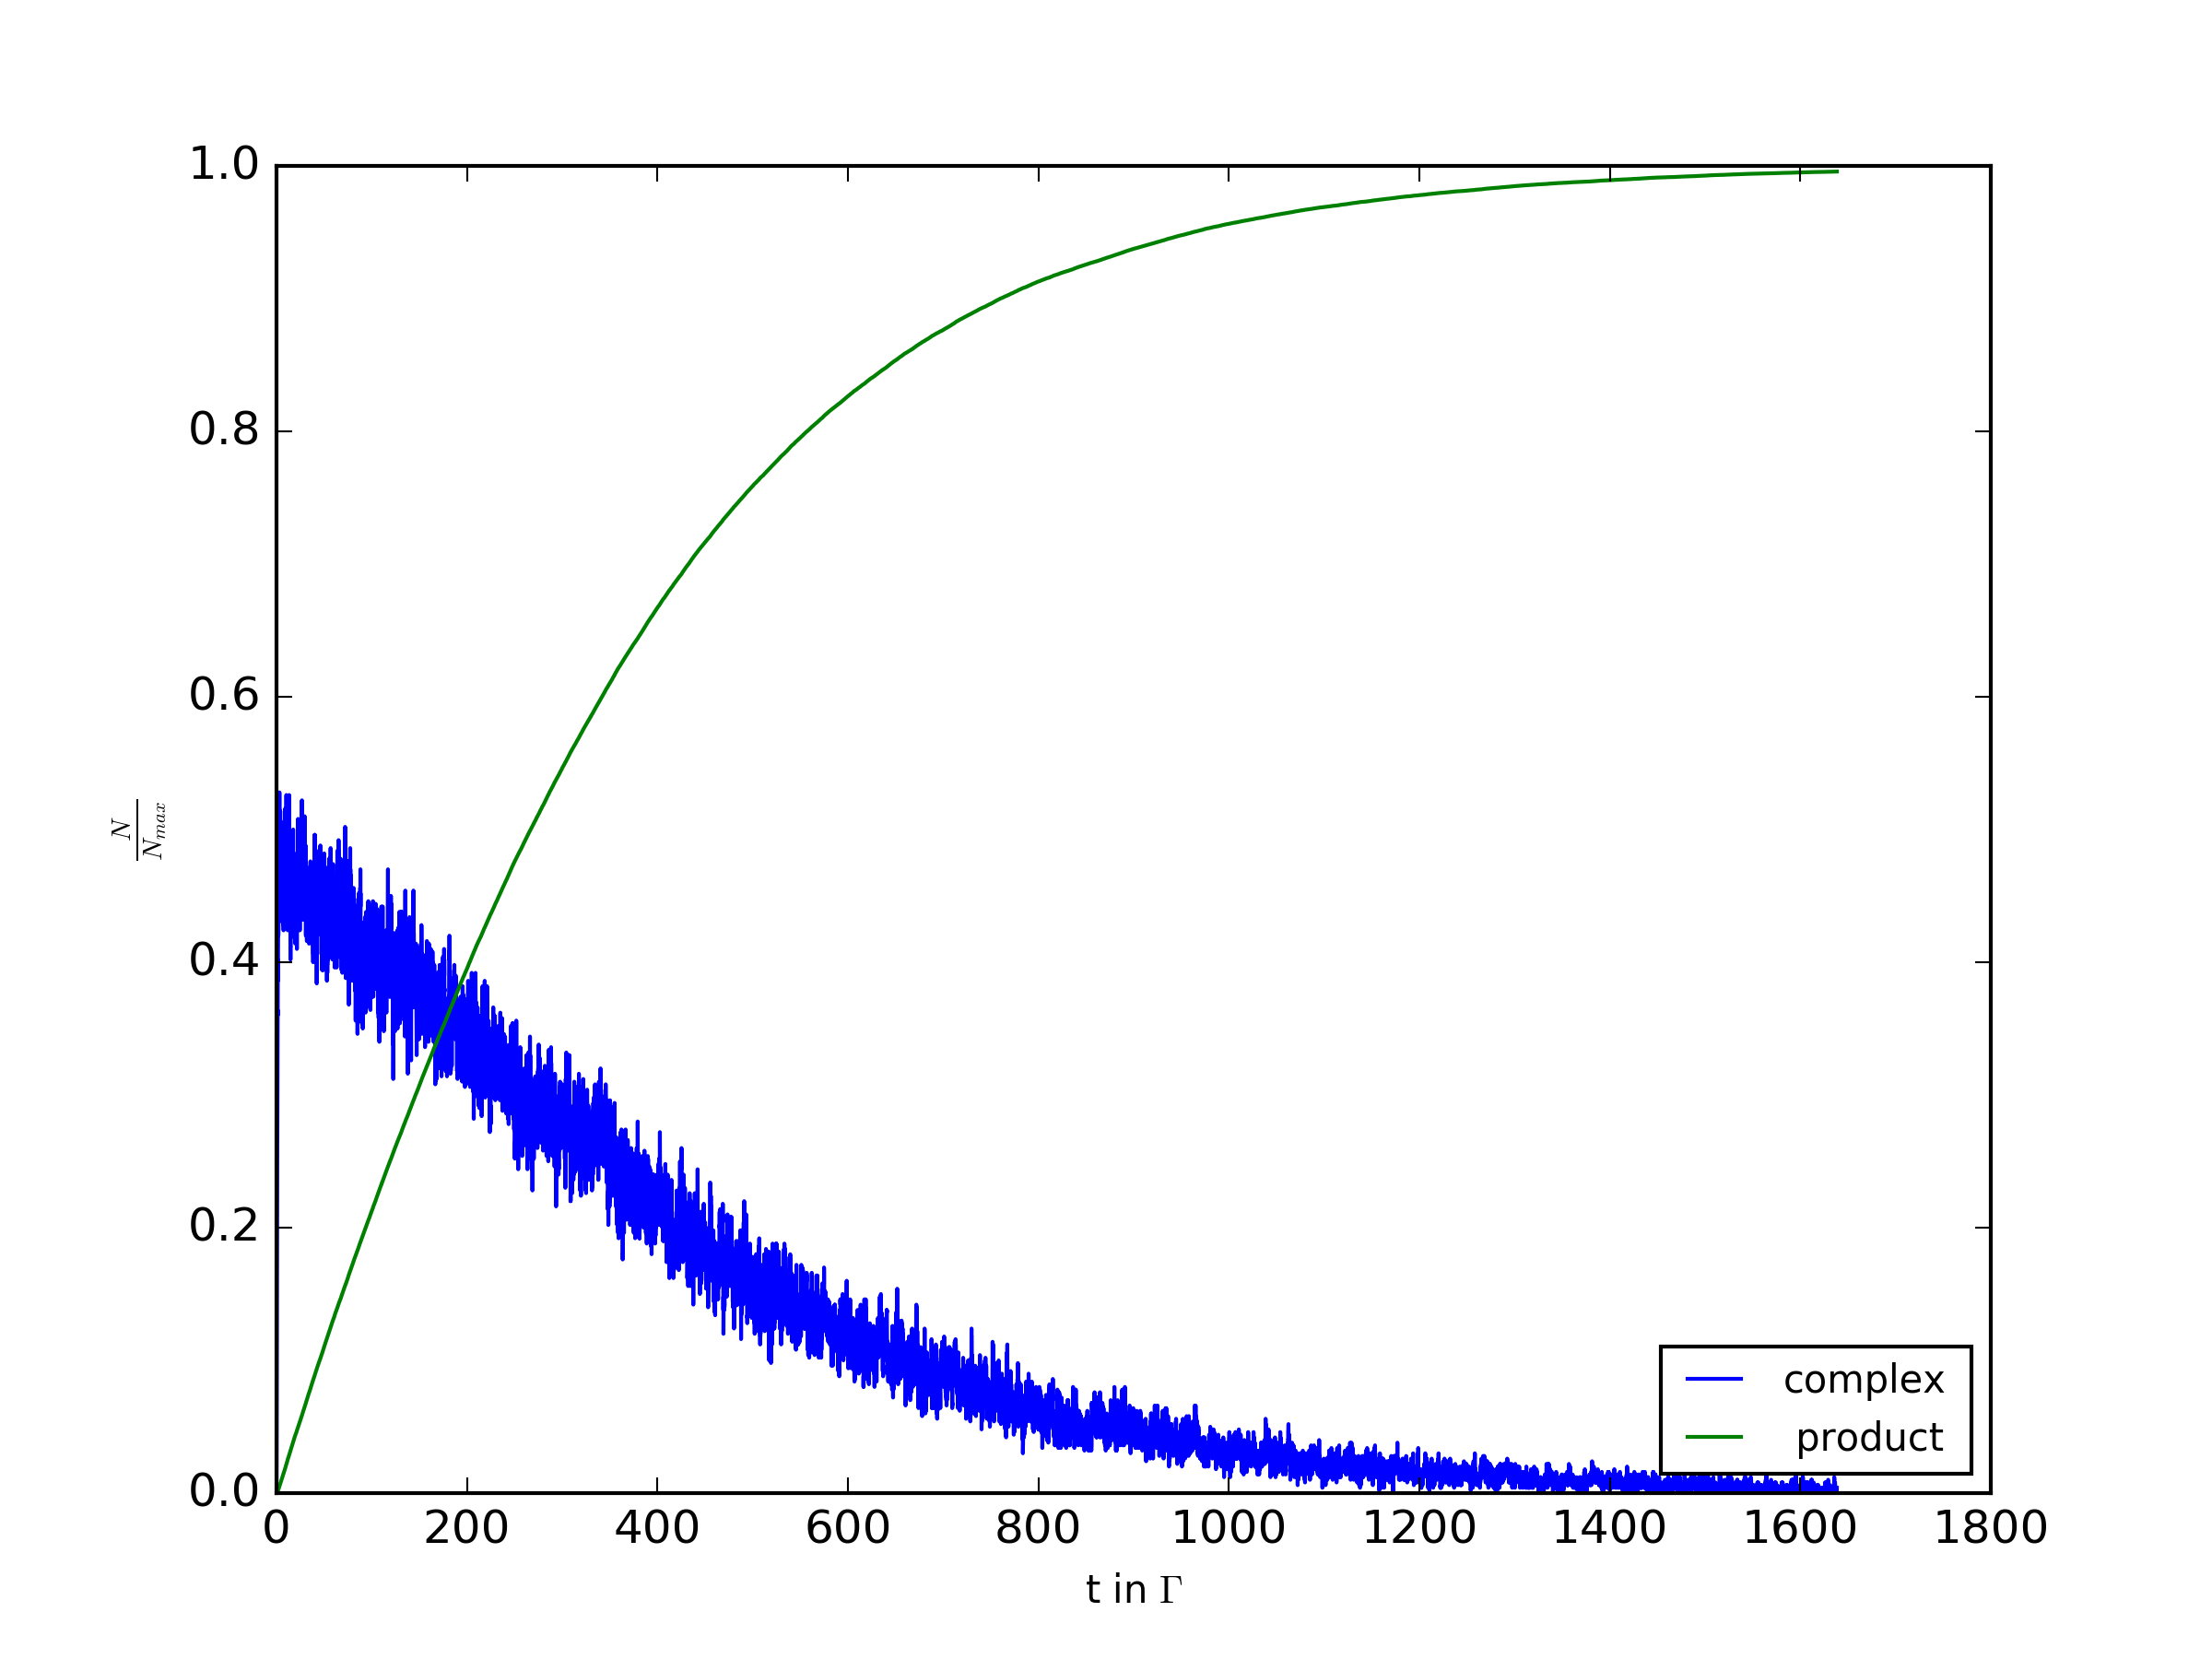
\includegraphics[width=\linewidth]{./data/profiling_length.png}
  \captionsetup{width=0.9\linewidth}
  \captionof{figure}{Scaling behaviour of computational time of both algorithms implemented in c++ and python  in respect to trajectory length $M$,for $N=1$, $t = \mathcal{O}(M log(M))$ }
  \label{fig:1}
\end{figure}
\begin{figure}[h!]
  \centering
  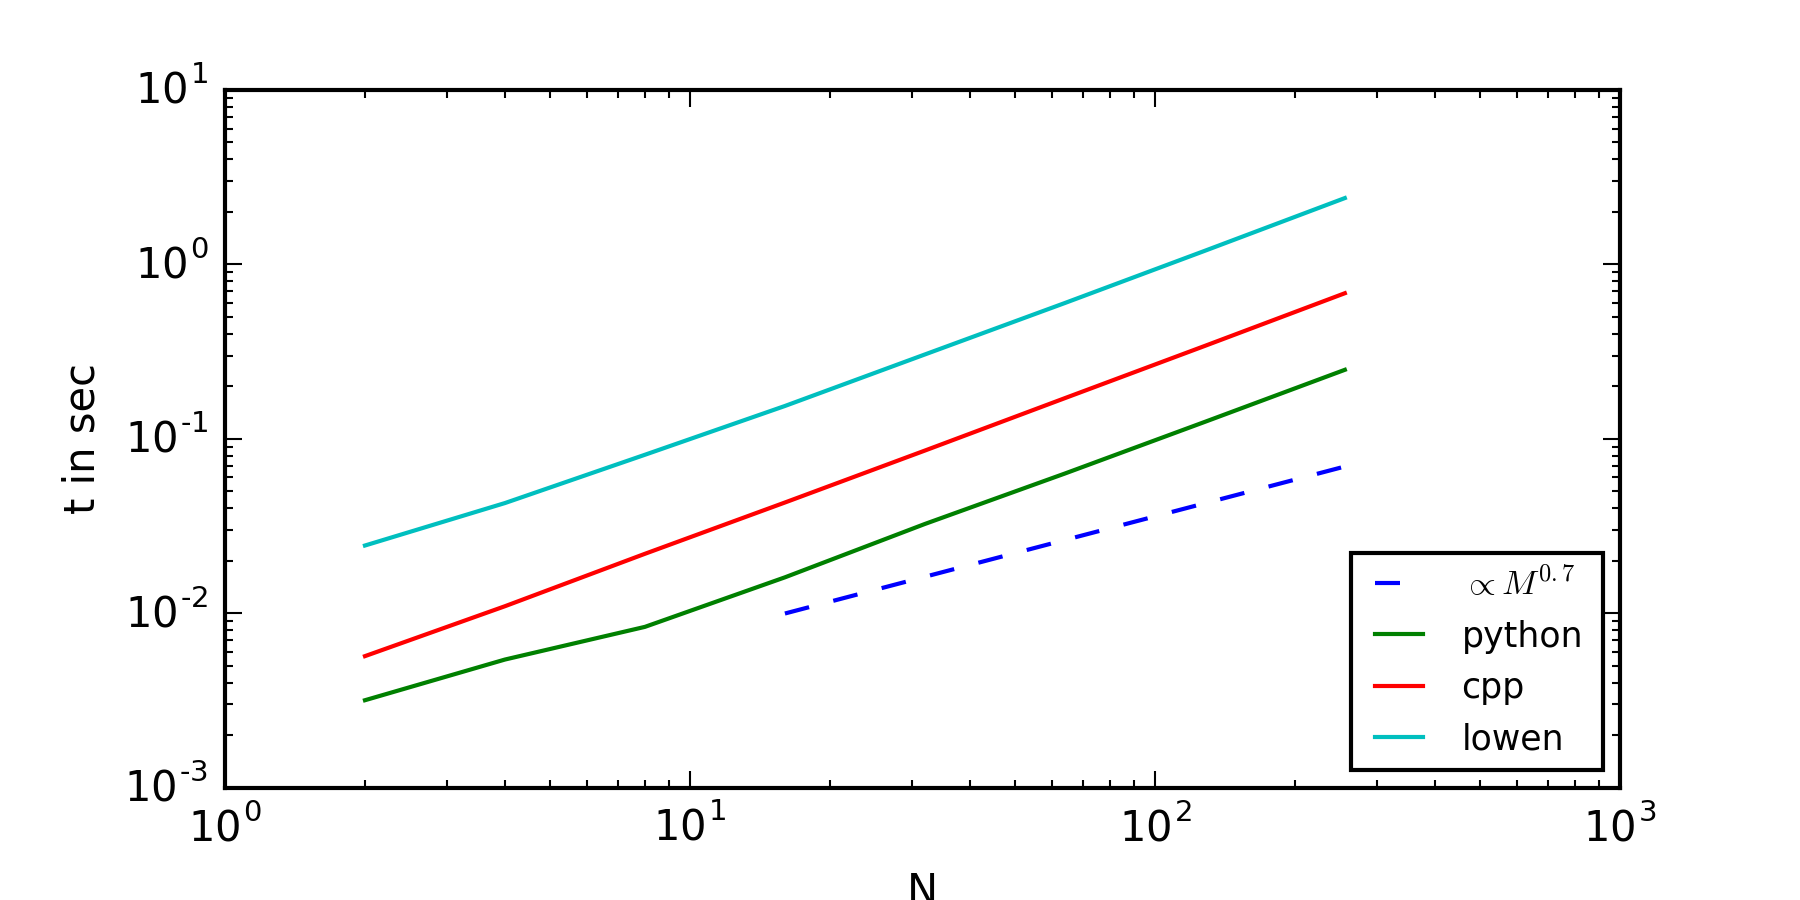
\includegraphics[width=\linewidth]{./data/profiling_particle.png}
  \captionsetup{width=0.9\linewidth}
  \captionof{figure}{Scaling behaviour of computational time of both algorithms implemented in c++ and python  in respect to trajectory number $N$ for $M=1000$ ,$t = \mathcal{O}(N log(N))$}
  \label{fig:2}
\end{figure}
\end{comment}
$t = \mathcal{O}(N))$ scaling
\begin{figure}[h!]
  \centering
  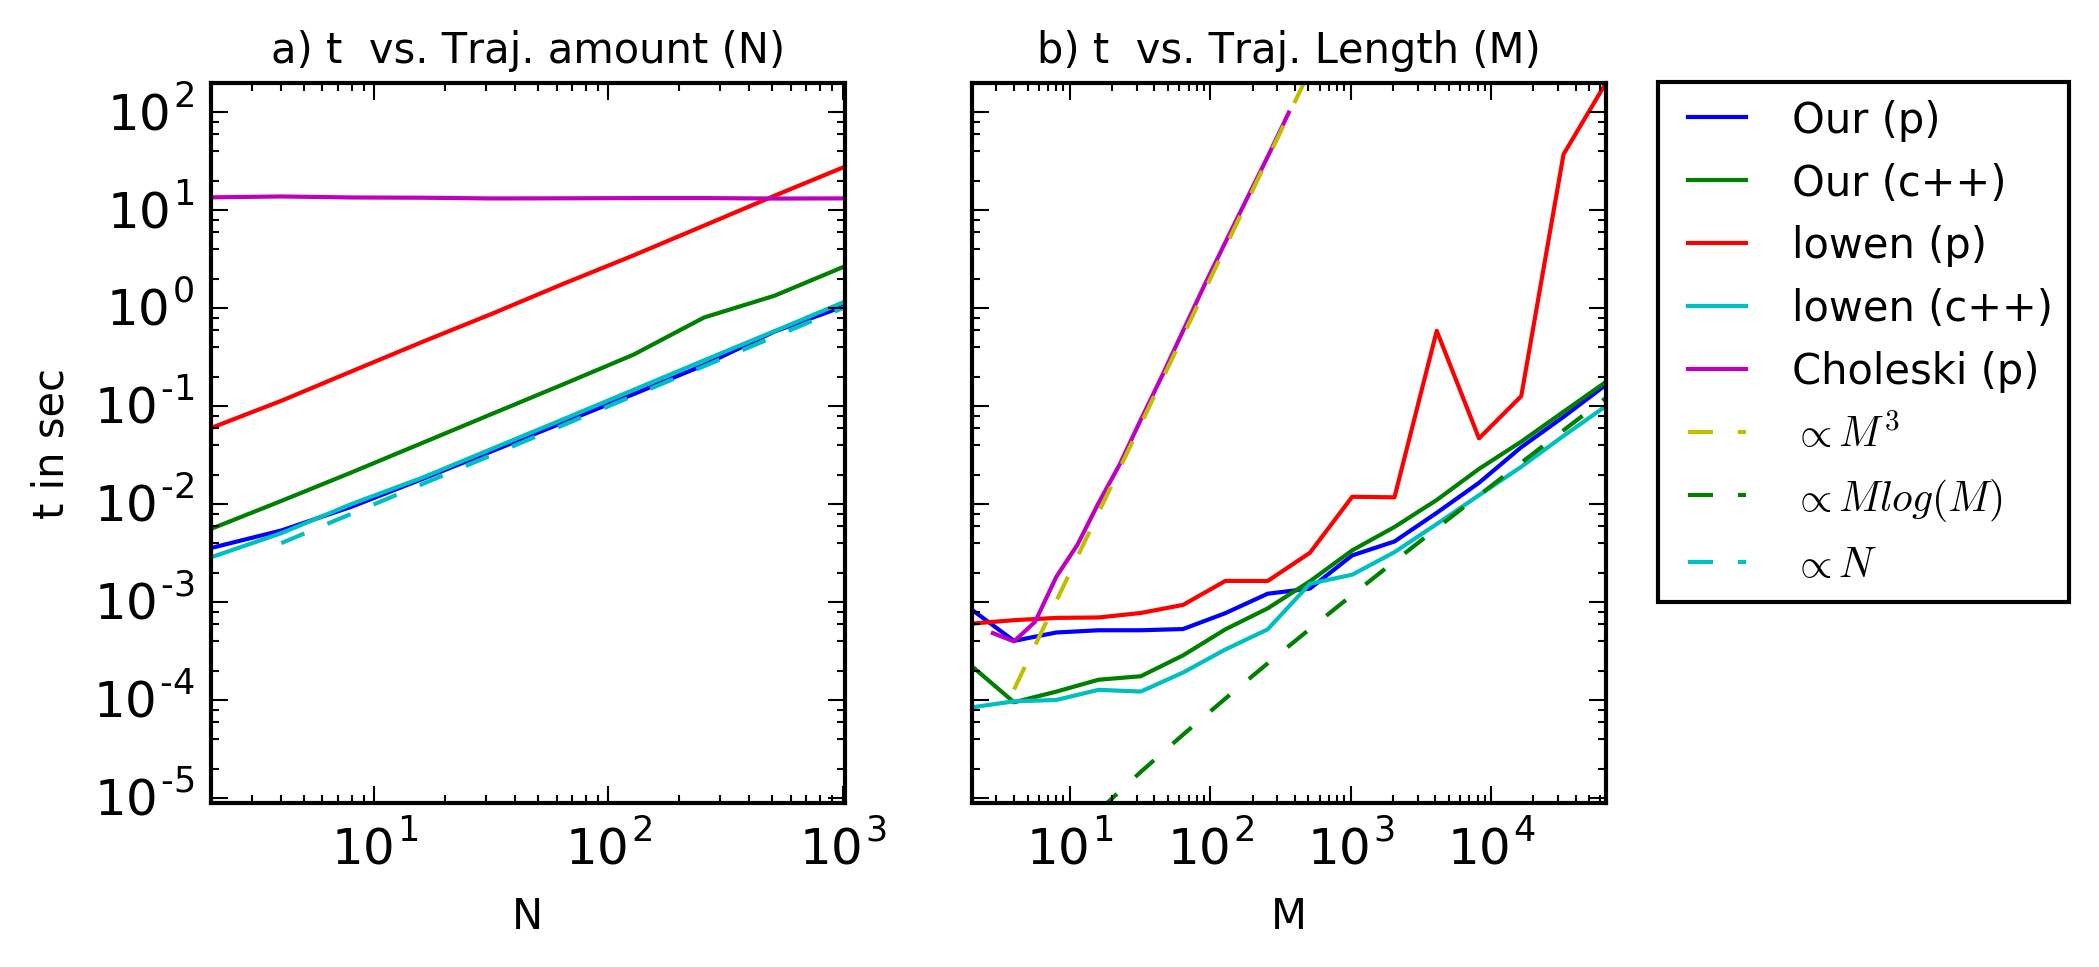
\includegraphics[width=\linewidth]{./data/profilingneu1.png}
  \captionsetup{width=0.9\linewidth}
  \captionof{figure}{a) Algorithmic scaling of computational time in respect to the amount of trajectories $N$ for trajectory length $M=1000$ , ($D=2$, $\alpha=0.5$, $\Delta t=1$) of Lowen and our own algorithm. Both implemented in  c++ and python (p) and the Choleski algorithm with $M=128$ implemented in python.\newline
  b) Algorithmic scaling of computational time in respect to the trajectory length $M$ for a single trajectory $N=1$ , ($D=2$, $\alpha=0.5$, $\Delta t=1$). Lowen and our own algorithms are implemented in c++ and python (p). Choleski is only implemented in python (p).}
  \label{fig:200}
\end{figure}
\noindent Subsequently also the non-Gaussian parameter was analyzed. For a perfect Gaussian process it should be zero as it is shown in \cref{nongaussian2}. \newline
Finally the algorithmic scaling was tested. FFT in python and c++ should scale for large number as  $\mathcal{O}(M log(M))$, which seams to be the cause for this algorithm as one can see in \cref{fig:200}. Further also the computational time(t) dependence on trajectories (N) were profiled as one can see in \cref{fig:200}.Again $t = M^{0.7}$ for large N.  
\chapter{Particle Based Reaction Diffusion}
This chapter is going to discuss particle based reaction diffusion. Particle based reaction diffusion is going to be put in relation to different reaction diffusion studying methods.  
Analytical solutions for resulting ordinary differencial equation exist under certain conditions like Quasi-Steady-State assumption or equilibrium assumption. In any case the mass action law is assumed. For fractional diffusion mass action law does not apply. Thus concentration based models had been upgraded by time depended rate coefficients \cite{Berry2002}  \cite{schnell2004reaction}
\section{Smoluchowski}
\section{Erban Chapmann}
\section{RevReaddy}
\chapter{An Enzymatic Reaction With Fractional Brownian Motion}
\section{Michaelis Menten}
\section{Simulation Model}
\section{Results From Normal Diffusion}
\section{Results from fBm}
\begin{figure}[h!]
  \centering
  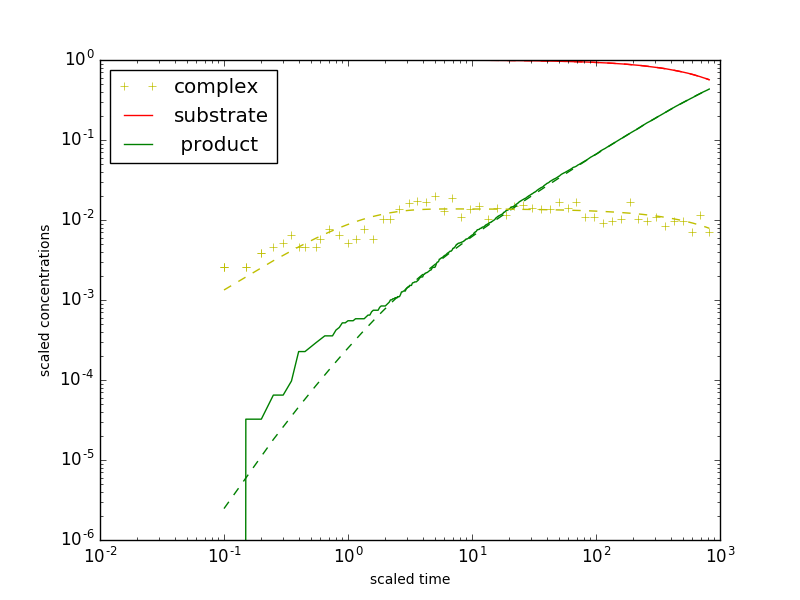
\includegraphics[width=\textwidth]{./data/erban-chapman-limit-concentrations1.png}
  \captionsetup{width=\linewidth}
  \captionof{figure}{ Erban Chapmann Concentrations}
  \label{fig:diffusion_limit-Erban-Chapmann}
\end{figure}
\begin{figure}[h!]
  \centering
  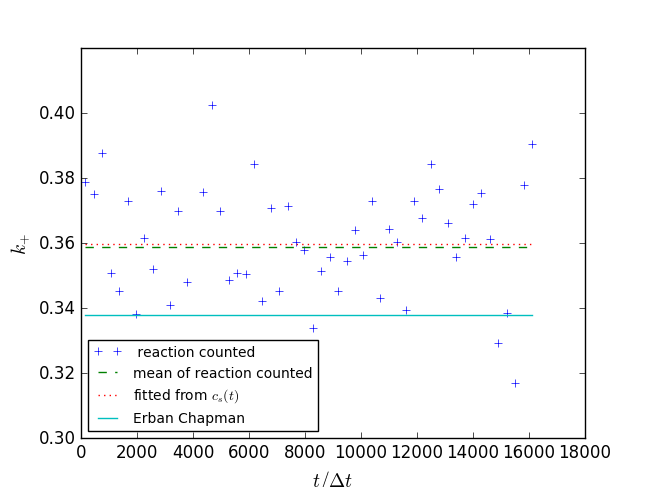
\includegraphics[width=\textwidth]{./data/chapman-limit-concentrations1_k1.png}
  \captionsetup{width=\linewidth}
  \captionof{figure}{ Erban Chapmann $k1$}
  \label{fig:diffusion_limit-Erban-Chapmann_k1}
\end{figure}

\begin{figure}[h!]
  \centering
  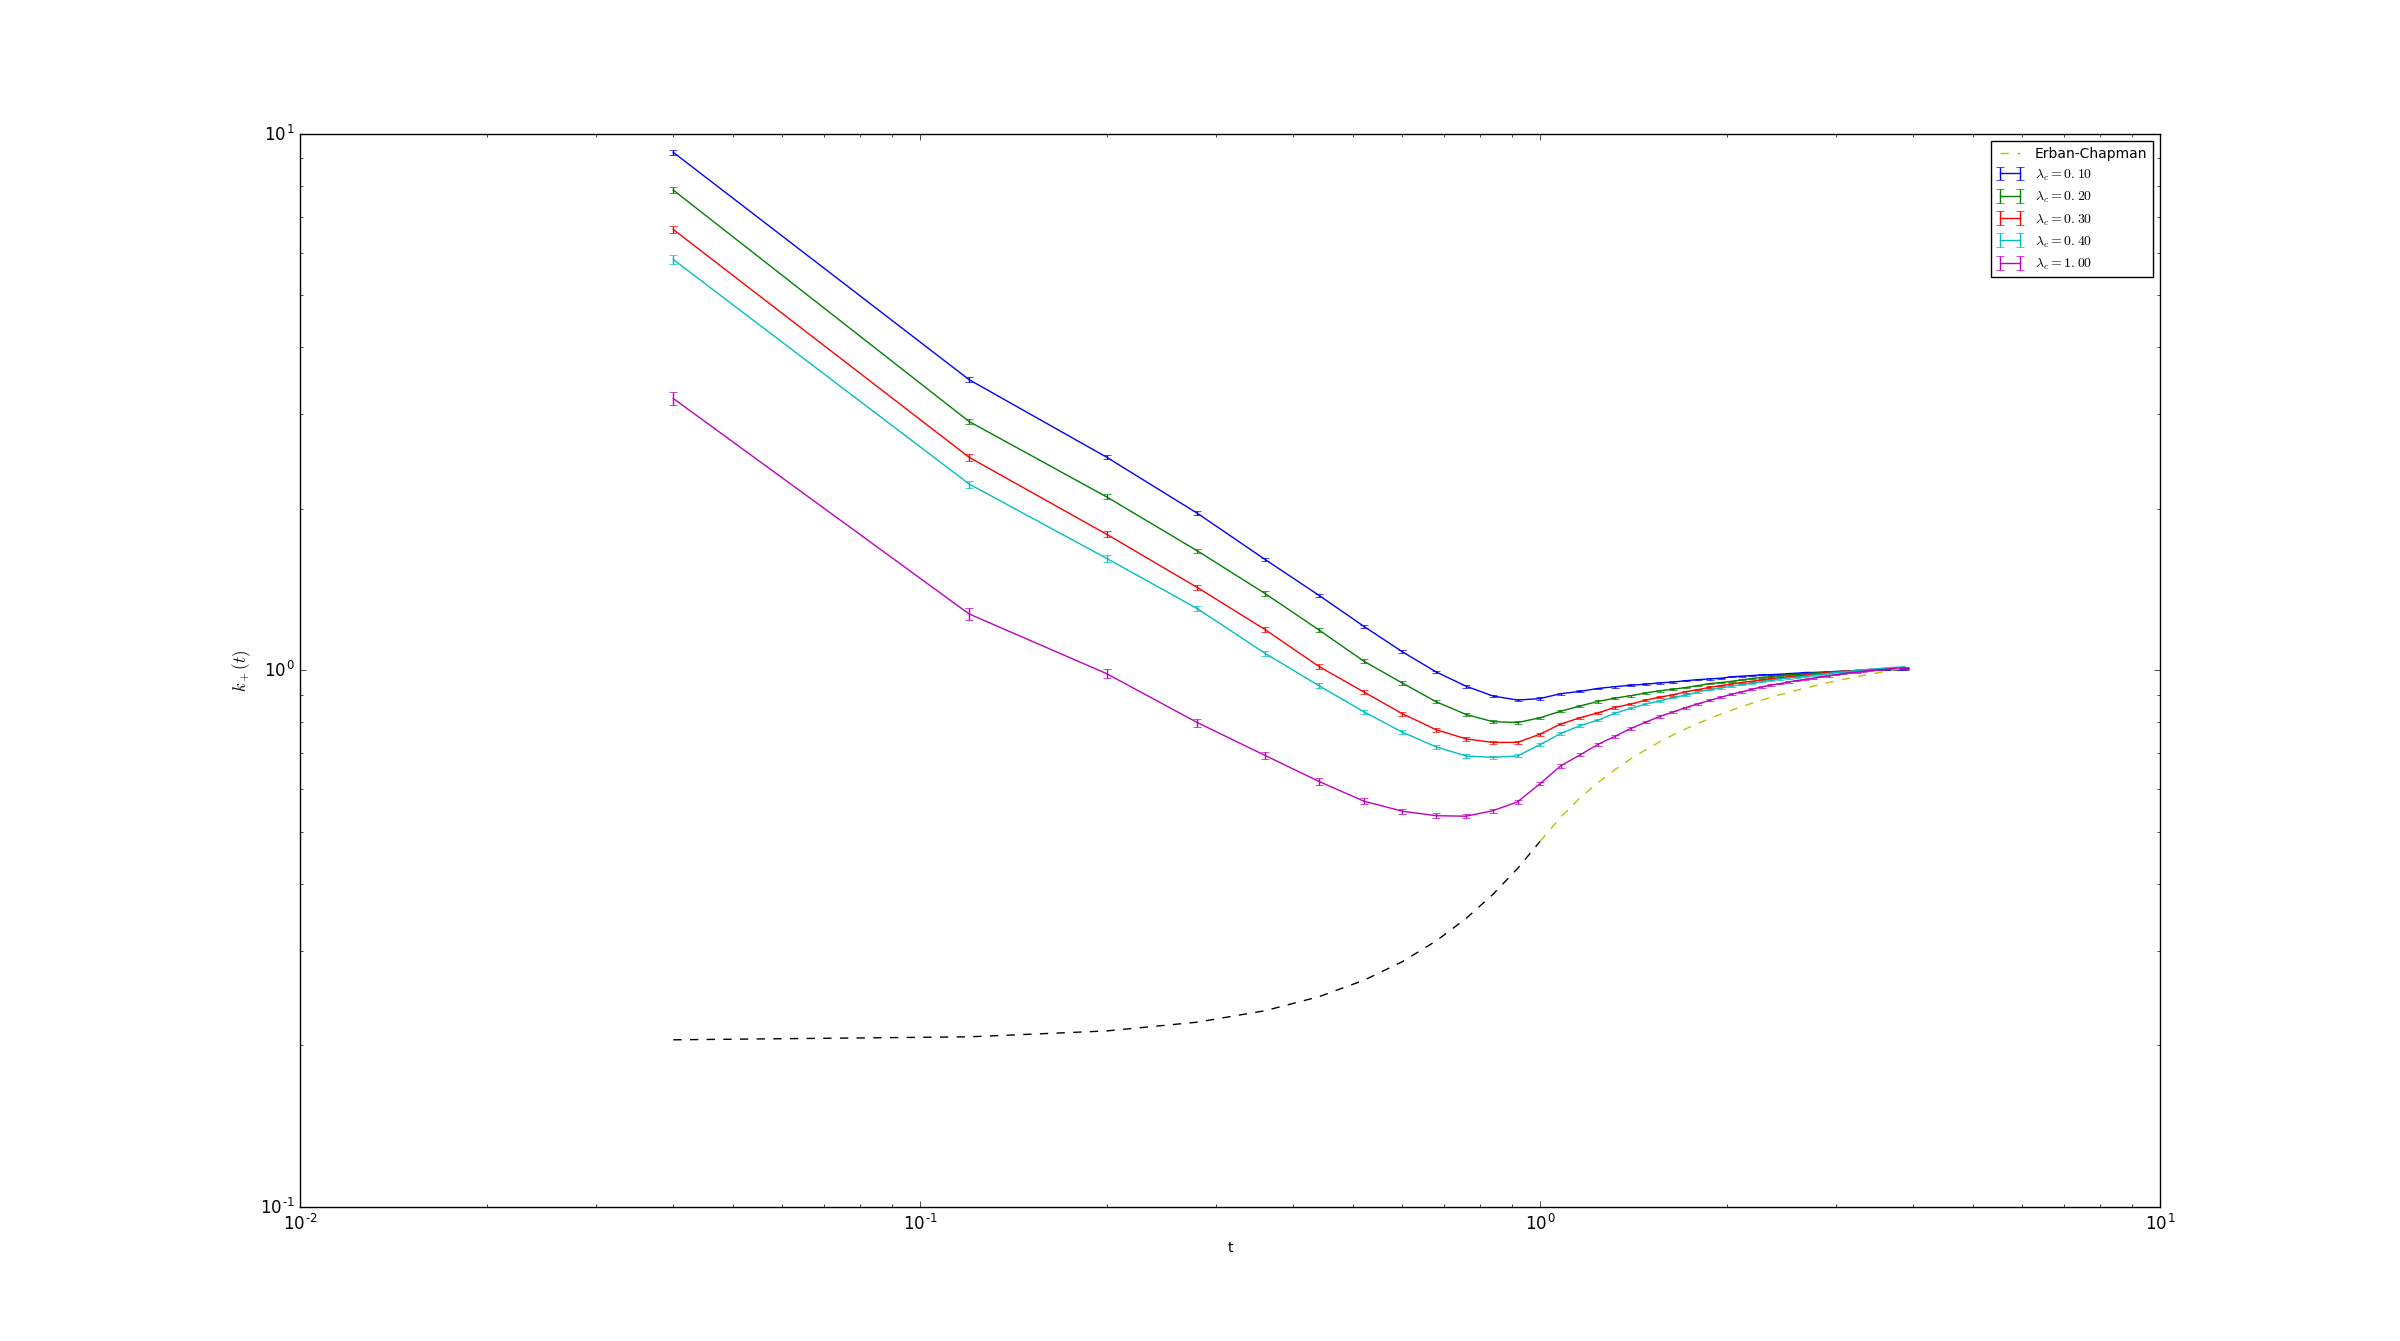
\includegraphics[width=\textwidth]{./data/microrate_complex_radial_erban.png}
  \captionsetup{width=\linewidth}
  \captionof{figure}{ Radial distribution for differnt $k_{c}$ }
  \label{fig:microrate_complex_radial_erban}
\end{figure}
\newpage

\begin{figure}[h!]
  \centering
  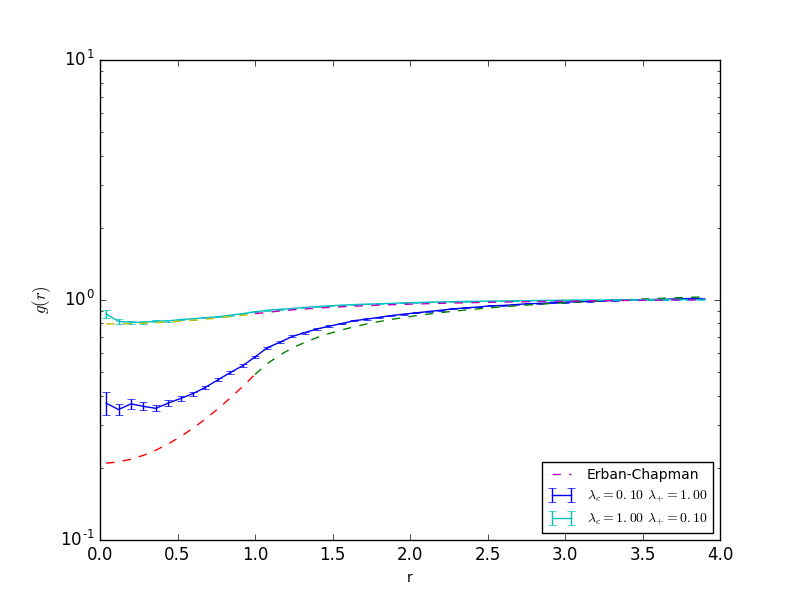
\includegraphics[width=\textwidth]{./data/microrate_complex_vsmicrorate_forward_radial_erban.png}
  \captionsetup{width=\linewidth}
  \captionof{figure}{ Radial distribution for $\lambda_{-}=0$ }
  \label{fig:microrate_complex_vsmicrorate_forward_radial_erban}
\end{figure}
\newpage


\begin{figure}[h!]
  \centering
  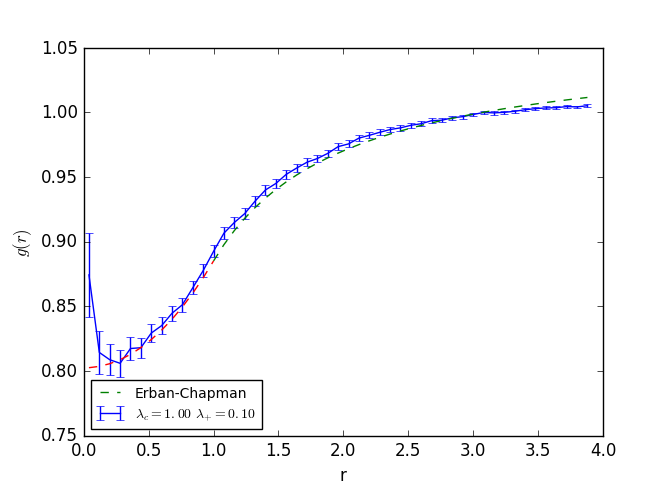
\includegraphics[width=\textwidth]{./data/chapman-limit-radial.png}
  \captionsetup{width=\linewidth}
  \captionof{figure}{ Erban Chapmann radial distribution}
  \label{fig:diffusion_limit-Erban-Chapmann_radial}
\end{figure}

\begin{figure}[h!]
  \centering
  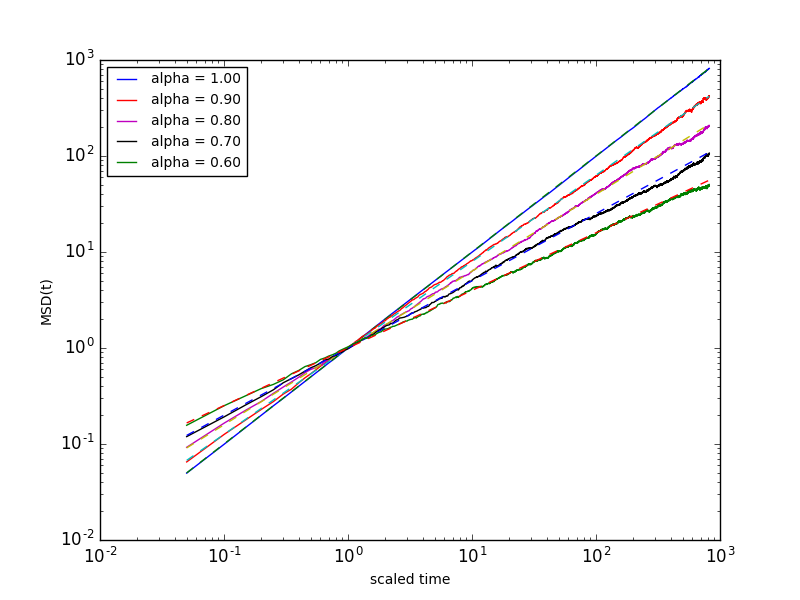
\includegraphics[width=\textwidth]{./data/differentalphamsdrevreaddy.png}
  \captionsetup{width=\linewidth}
  \captionof{figure}{ different alpha}
  \label{fig:differentalpharevreaddymsd}
\end{figure}

\begin{figure}[h!]
  \centering
  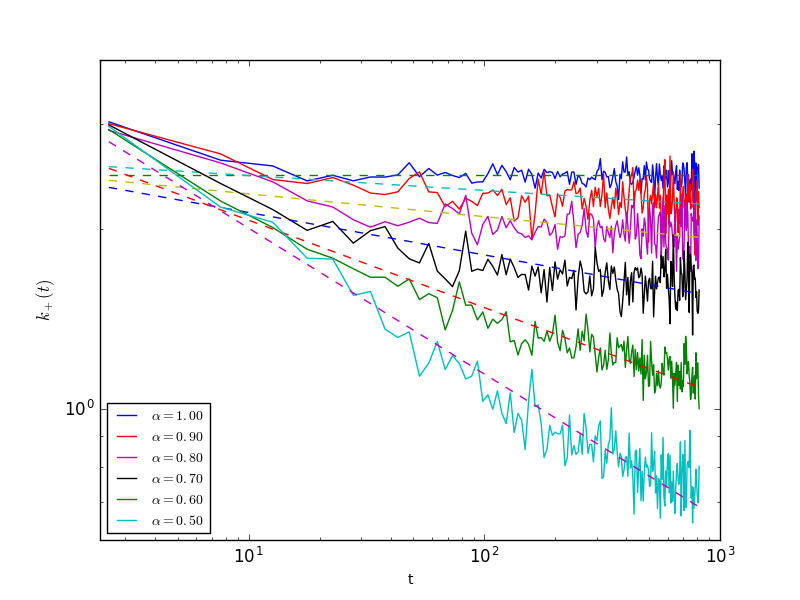
\includegraphics[width=\textwidth]{./data/k1_fordifferentalpha_withfit.png}
  \captionsetup{width=\linewidth}
  \captionof{figure}{$k1(t)$ for differnt $\alpha$ with fitted h}
  \label{fig:k1differentalphawithfit}
\end{figure}

thesis: $k1(t)\propto t^{-h}$

\section{Conclusion}
\chapter{Summary}
\chapter{Appendix}
\section{From Central Limit Theorem to Gaussian Distribution}\label{append:CLT}
In the following the Central Limit Theorem will be applied to calculated the distribution of Y,  $\rho(y)dy=P(y<Y<y+dy)$ in the limit of large N , with Y being defined as the sum of an random variable:
 \begin{align}
  Y = \frac{1}{\sqrt{N}} \sum_{j=1}^N X_j \label{eq:CLT1}
 \end{align}
The Generating function for a random variable $Y$ is: 
\begin{align}
 G_Y(k)=\langle e^{ikY}\rangle = \int e^{ikY} \rho(y)dy
\end{align}
\cref{eq:CLT1} can be inserted into the generating function, which results in:
\begin{align*}
G_Y(k)=\langle e^{\frac{ik}{\sqrt{N}} \sum_{j=1}^N X_j}\rangle \\
G_Y(k)=\langle \prod_{j=i}^N e^{\frac{ik}{\sqrt{N}} X_j} \rangle 
\end{align*}
If all $X_j$ are independent, then:
\begin{align}
 G_Y(k)= \prod_{j=i}^N \langle e^{\frac{ik}{\sqrt{N}} X_j} \rangle =e^{\sum_{j=1}^N A_j (\frac{k}{\sqrt{N}})} \\ \nonumber \text{ with } A_j(\frac{k}{\sqrt{N}})= ln \langle e^{\frac{ik}{\sqrt{N}} X_j} \rangle 
\end{align}
For large N behavior, we assume $\frac{k}{\sqrt{N}} << 1$ and expand
\begin{align}
 A_j(\frac{k}{\sqrt{N}}) = ln(1+ \langle X_j \rangle \frac{ik}{\sqrt{N}} - \langle X_{j}^2 \rangle \frac{k^2}{2N}+\mathcal{O}(N^{- \frac{3}{2}}))
\end{align}
 with a finite variance $ \sigma_i^2=\langle X_{i}^2\rangle $ and the mean $\langle X_{i}\rangle = 0$
\begin{align}
 A_j(\frac{k}{\sqrt{N}}) = -\sigma_j^2 \frac{k^2}{2N}+\mathcal{O}(N^{- \frac{3}{2}}))
\end{align}

Thus, the generating function for large N is:

\begin{align}
 G_Y(k)=e^{- \frac{\sigma^2 k^2}{2}} \\ \nonumber
 \text{ with } \sigma =  \frac{1}{N} \sum_{j=1}^N \sigma_j^2 
\end{align}
The distribution of Y can be calculated via the inverse Fourier Transform:
\begin{align}
 \rho(y) &=\frac{1}{2 \pi} \int_{-\infty}^{\infty} e^{- \frac{\sigma^2 k^2}{2}} e^{i k y} dk \\  
 &=\frac{1}{\sqrt{2 \pi} \sigma } e^{-\frac{y^2}{2 \sigma^2}}
\end{align}
$\rho(y)$ results in a Gaussian distribution.

\section{From Gaussian Distribution to Gaussian Transition Probability}\label{baystheorem}
The conditional distribution function to be in $x$ at time $t$ if visited position $y$ at time $s$   can be written due to Bayes' theorem as a transition probability from $y$ to $x$ in time $t-s$ multiplied with the probability to be in $y$ at time $s$:
\begin{align}
 \rho_{t,s}(x,y)=T_{t-s}(x|y) \rho_s(y)
\end{align}
Further due to particle conservation another relation holds:
\begin{align}
 \rho_{t}(x)= \int \rho_{t,s}(x,y) dy
\end{align}
Having an initial condition $\rho_{s}(x)= \delta(x-y)$:
\begin{align}
 \rho_{t,s}(x|y)&= \int \rho_{t,s}(x,y) dy = \int T_{t-s}(x|y) \rho_s(y) dy\\
 &= \int T_{t-s}(x|y) \delta(x-y) dy 
 = T_{t-s}(x|y)
\end{align}
\section{Einstein Formula} \label{einsteinrealtionappendix}
The derivative of the mean variance of the Gaussian distribution in respect to time is defined as:
\begin{align}
 \frac{d}{dt}  \delta \bm{r}^2(t)&=\frac{d}{dt} \langle \Delta \bm{ R}^2(t)\rangle  =\frac{d}{dt} \int d\bm{r} \bm{r}^2 c(\bm{r},t)=\int d\bm{r} \bm{r}^2 \frac{\partial}{\partial t} c(\bm{r},t) 
\end{align}
Fick's second law can be applied:
\begin{align}
&= D \int_{-\infty}^{\infty}d\bm{r} \bm{r}^2 \Delta c(\bm{r},t)  
\end{align}
Assuming a reasonable assumption  $c(\pm \infty,t)=0$  and two times partial integration one can derive:
\begin{align}
&= -2 D \int_{-\infty}^{\infty} d\bm{r} \bm{r} \nabla c(\bm{r},t) \\ &= 2 D d \int_{-\infty}^{\infty} d\bm{r} c(\bm{r},t) =2dD
\end{align}
For the initial condition $\bm{r}(0) = 0$,  one gets the Einstein Formula: $\langle (\bm{r}(t)-\bm{r}(0))^2)\rangle= 2dDt$
\begin{comment}
check book zwanzig
\end{comment}
\section{Autocorrelation Function for fBm}\label{VACF}
Subsequently, the VACF in the frequency domain for Fractional Brownian motion can be calculated. The MSD is $\delta r^{2}(t)= < \Delta R(t)>=2dK_{\alpha}t^{\alpha}$ with $K_{\alpha}$ being the generalized diffusion-coefficient:
\begin{align*}
 \tilde{Z}(z)&=\int_{0}^{\infty} d t e^{izt} Z(t) \\
 &=\frac{1}{2 d} \int_{0}^{\infty} d t e^{izt} \left[\frac{d^2}{dt^2}\delta r^2 (t) \right]
\end{align*}
Partial integration:
\begin{align*}
  \stackrel{par. integ.}{=} \frac{1}{2 d} \left( \underbrace{\left [ e^{izt}\overbrace{ \frac{d}{dt} 2dK_{\alpha}t^{\alpha}}^{=A(t)} \right]_{0}^{\infty}}_{\stackrel{\alpha < 2} {=} 0}- i z \int_{0}^{\infty} d t e^{izt} \left[\frac{d}{dt}\delta r^2 (t)\right] \right) 
 \end{align*}
 \begin{align*}
 A(t)=\frac{d}{dt}\overbrace{ \left [\frac{2d K_{\alpha}t^{\alpha-1}}{\alpha} \right ]}^{B(t)}=\frac{2d K_{\alpha}t^{\alpha-2}}{\alpha+(\alpha-1)}
\end{align*}

Partial integration and Tauber theorem:

\begin{align*}
 \tilde{Z}(z) & \stackrel{par. integ.}{=} - \frac{1}{2 d} \left( \underbrace{\left [ e^{izt}\overbrace{  2dK_{\alpha}t^{\alpha}}^{=B(t)} \right]_{0}^{\infty}}_{\stackrel{\alpha < 1} {=} 0} - (iz)^2 \int_{0}^{\infty} d t e^{izt} \delta r^2 (t) \right) \\
  & = - \frac{z^2}{2 d}\int_{0}^{\infty} d t e^{izt} \delta r^2 (t)  \stackrel{\operatorname{Im}(z)> 0} {=}  K_{\alpha} \Gamma(1+\alpha)(i z)^{1-\alpha} 
\end{align*}

\section{Kinetics of the Bi-Molecular Chemical Reaction in Solution}\label{bi-molecular}
The aim of this calculation is to derive the kinetics for the following reaction scheme: \ch{A + B <>[ $k^{+}_{\mathrm{d}}$ ][ $k^{-}_{\mathrm{d}}$ ] AB }\newline
The derivation is calculated under the assumption of free diffusion of particle A and B with the diffusion constants $D_A$ and $D_B$ , respectively and without any interactions between them. 
The joint concentration field can be described by the Smoluchowski equation for a bi-molecular system in a solution:
\begin{align}
 \frac{\partial \rho_t(\bm{r}_A,\bm{r}_B)}{\partial t}=(D_A \nabla^{2}_{A}+D_B \nabla^{2}_{B}) \rho_t(\bm{r}_A,\bm{r}_B) \label{smolubi}
\end{align}
The complexity of the problem can be reduced by substituting the positions of the particles A and B with their relative distance $\bm{r}=\bm{r}_A-\bm{r}_B$. It is convenient to introduce even further substitutions:
\begin{align}
 D= D_A+D_B \qquad \qquad \bm{R}=\frac{D_B \bm{r}_A+ D_A \bm{r}_B}{D_A+D_B}
\end{align}
the Laplace operator in terms of new coordinates result in:
\begin{align}
\nabla^{2}_{A} = \left( \nabla_r+\frac{D_B}{D} \nabla_R \right)^2 \\
\nabla^{2}_{B} = \left( \nabla_r+\frac{D_A}{D} \nabla_R \right)^2 
\end{align}
Inserting these in \cref{smolubi} one gets:
\begin{align}
 \frac{\partial \tilde{\rho}_t(\bm{r},\bm{R})}{\partial t}=\left(D \nabla^{2}_{r}+\frac{D_B D_A}{D_A+D_B}\nabla^{2}_{R}\right) \tilde{\rho}_t(\bm{r},\bm{R})
\end{align}
The equation is describing two independent diffusion processes, one in
the coordinate $\bm{r}$ and one in the coordinate $\bm{R}$. The solution can be obtained by the product ansatz $\tilde{\rho}_t(\bm{r},\bm{R})=\rho_t(\bm{r})q_t(\bm{R})$. Integration over $\bm{R}$ results in:
\begin{align}
\frac{\partial \rho_t(\bm{r})}{\partial t}=D \nabla^{2}_{r} \rho_t(\bm{r}) +\frac{D_B D_A}{D_A+D_B} \nabla^{2}_{R} \rho_t(\bm{r}) \int_{\partial V} q_t(\bm{R}) d \bm{a}
\end{align}
In the previous equation the stokes theorem was applied. The second term is zero due to conservation of probability. The problem is isotropic, hence $r=|\bm{r}|$ and $\nabla^{2}_{\bm{r}}=\left(\partial_r+\frac{2}{r}\right)\partial$. The equation reduce to one dimension:
\begin{align}
\frac{\partial \rho_t(r)}{\partial t}=-\left(\frac{\partial}{\partial_r}+\frac{2}{r} \right) j_t(r) \qquad \qquad j_t(r)=D \frac{\partial\rho_t(r)}{\partial_r}
\end{align}
 The stationary distribution results in:
\begin{align}
 0 &=-\left(\frac{\partial}{\partial_r}+\frac{2}{r} \right) j^{s}_t(r) \\
 \frac{d j^{s}_t(r)}{j^{s}_t(r)}  &=- \frac{2}{r} dr\\
 j^{s}_t(r)&=A r^{-2}\\
 \rho^s(r)&=\rho^s(r_0)- \frac{\int_{r_0}^{r} j^{s}_t(r')dr'}{D}=\rho^s(r_0)+\frac{A}{D}\left(\frac{1}{r}-\frac{1}{r_0}\right)
\end{align}
Now assuming only a single B molecule being at the position $r=0$. Instantaneous reaction occur for $r\leq \sigma \Rightarrow \rho_t(r \leq \sigma)=0$. For $r \rightarrow \infty$ the distribution is than defined as the concentration of particle A $\rho_t(r \rightarrow \infty)=c_A$ and 
the Solutions for $\rho^{s}(r)$ and $j^{s}_t(r)$ for the boundary conditions are:
\begin{align}
 \rho^{s}(r)=C_A \left(1-\frac{\sigma}{r}\right) \qquad j^{s}_t(r)&=-D \sigma C_A r^{-2}
\end{align}
The change of the concentration of $C_{AB}$ is then: 
\begin{align}
 \frac{d C_{AB} }{d}=4 \pi \sigma D C_A C_B
\end{align}
By formulating the problem in relative distance from particle A and B. It was also reasonable to keep particle B at its initial position. The results shows the relation between the product of the concentrations and the concentration change.In the derivation of Michealis-Menten kinetics this is an assumption. 



\section{Michaelis-Menten Kinetics}\label{Menten_der}
Michaelis-Menten kinetics are describing the following system:\newline
\ch{S + E <>[ $k_{\mathrm{1}}$ ][ $k'_{\mathrm{1}}$ ] E S -> [ $k_{\mathrm{2}}$ ] P + E}.
A range of differential equations can be formulated as a result of particle conservation and the assumption for a bi-molecular chemical reaction to be proportional to the product of the reactants concentration. 
\begin{align}
\frac{d[P]}{dt} &= k_{\mathrm{2}} [ES] \\ \label{first}
\frac{d[E]}{dt} &= k_{\mathrm{2}} [ES]+k'_{\mathrm{1}} [ES]-k'_{\mathrm{1}} [E][S]\\
\frac{d[S]}{dt} &= k'_{\mathrm{1}} [ES]-k'_{\mathrm{1}} [E][S]\\
\frac{d[ES]}{dt} &=  - k_{\mathrm{2}} [ES] -k'_{\mathrm{1}} [ES]+k'_{\mathrm{1}} [E][S]
\end{align}
With a quasi-steady-state approximation: $\frac{d[ES]}{dt}=0  \longrightarrow k_{\mathrm{1}}[E][S]=k'_{\mathrm{1}}[ES]+k_{\mathrm{2}}[ES]$. A Rearrangement of this equation results in the  Michaelis-Menten constant: $K_M=\frac{k'_{\mathrm{1}}+k_{\mathrm{2}}}{k_{\mathrm{1}}}=\frac{[E][S]}{[ES]}$. From the enzyme conservation law one gets:
\begin{align}
[E]=[E]_0 -[ES] \label{conservationenym}
\end{align}
After inserting \cref{conservationenym} into the quasi-steady-state approximation, one gets:
\begin{align}
 [ES]=\frac{[E]_0 [S]}{K_M+[S]}
\end{align}
Combining it with the first differential \cref{first} one gets the rate of Product production:
\begin{align}
 v= \frac{d[P]}{dt}= k_{\mathrm{2}} \frac{[E]_0 [S]}{K_M+[S]} = V_{max} \frac{[S]}{K_M+[S]}  
\end{align}

\chapter{old stuff}
\section{Theory}
\subsection{Diffusion-controlled Reactions for Brownian Motion}
Chemical reactions are omnipresent in biological systems. Reactions are composed of reactants and products. These reactants and products are atoms or molecules with changing number over time during reactions. Studying chemical reactions often contains reaction kinetics. Reaction kinetics is about rates of chemical process. Enzymatic reactions e.g. play an important role in biological systems to reduce rates of reactions. The rates of reactions in solutions are not only governed by intrinsic reaction rates, which were addressed e.g. by Kramer's escape problem for two reactants, but also on rates at which the chemical participants diffuse into close proximity. In a reaction of the following type: \ch{A + B <>[ $k^{+}_{\mathrm{d}}$ ][ $k^{-}_{\mathrm{d}}$ ] AB <> [ $k^{+}_{\mathrm{a}}$ ][ $k^{-}_{\mathrm{a}}$ ] C}. \newline The Kramer's escape problem deals with the rates on the right side  $k^{\pm}_{\mathrm{a}}$. Smoluchowski deals with the rates on the other side $k^{\pm}_{\mathrm{d}}$. \newline  A theoretical approach on how fast two particles come together in a dilute system of hard spheres moving independently with Brownian motion have been studied by Marian von Smoluchowski in 1916 \cite{Smoluchowski1}. This was the first study on diffusion-limited reaction rates. A constant rate $k^{+}$ can be written as:
\begin{align}
 k^{+}=4 \pi (D_1+D_2)(R_1+R_2)=4 \pi (D_1+D_2) \sigma \label{reactionrate11}
\end{align}
with $\sigma = R_1+R_2$ the relative distance between the sphere centres.  It is a direct result of the diffusion equation. The calculation can be found in the appendix \ref{bi-molecular}. One particular area of research on which the Smoluchowski relation had significant impact in the last few decades is biology. This is unsurprising as a vast number of biomolecular systems involve dilute and minute diffusing molecular populations undergoing continuous reaction. Understanding how these biological systems operate is complicated and is in itself a whole field of research; systems biology. The Smoluchowski result has provided a very powerful tool for theoretical investigation of microscopic biochemical reaction-diffusion processes \cite{Flegg}. It was extended by P. Debye in 1942 to add intermolecular forces. However, especially in biological systems Brownian motion do not apply for all time-scales. As stated in the motivation these environments exhibit very often anomalous diffusion, which can be addressed by fBm. 
\newline
A related reaction type was studied by L. Michaelis and Maud L. Menten in 1913 \cite{Johnson2011}. Also Known as Michaelis-Menten kinetics:   
\ch{S + E <>[ $k_{\mathrm{1}}$ ][ $k'_{\mathrm{1}}$ ] E S <> [ $k_{\mathrm{2}}$ ] [ $k'_{\mathrm{2}}$ ]P + E}, with $k'_{\mathrm{2}}=0$. The assumption of irreversibility can be considers as a good approximation, if the concentration of the substrate  is a lot larger then the concentration of the Product $[S]\gg[P]$ or if the Gibbs free energy (released energy) is very large  $\Delta G \ll 0$ (Kramer's escape Problem). With a further quasi-steady-state approximation  ($k_{\mathrm{1}}[E][S]=k'_{\mathrm{1}}[ES]+k_{\mathrm{2}}[ES]$) the Michaelis-Menten equation results in:
\begin{align}
 v= \frac{d[P]}{dt}=V_{max} \frac{[S]}{K_M+[S]}  \qquad \text{ with } \qquad K_M=\frac{k'_{\mathrm{1}}+k_{\mathrm{2}}}{k_{\mathrm{1}}}
\end{align}
The derivation can be found in the appendix \ref{Menten_der} . In the first step the relation $\frac{d[ES]}{dt}\propto [E][S]$ is assumed. This is coherent with the results from the calculation for kinetics of bi-molecular reaction in solutions with the assumption of normal diffusion in \cref{bi-molecular}. However, in the environment of a living cell where there is a high concentration of proteins, the cytoplasm often behaves more like a gel than a liquid, limiting molecular movements and altering reaction rates \cite{Zhou2008}.

\begin{comment}
 Belousov-Zhabotinsky-Reaktion ?
 https://en.wikipedia.org/wiki/Reaction%E2%80%93diffusion_system interessint 
 Two-component reaction–diffusion equations
\end{comment}
\section{Simulation and Outlook}
A software package revReaDDy was used to simulate reactions in a dilute system. It builds upon ReaDDy \cite{Johannesschoneberg2014} and is still under development. It is a particle based simulation software acting on a macromolecular level. For the following simulation Brownian motion was used as an integrator and will be replaced by fBm in the second half of the master thesis. RevReaDDy has periodic boundary conditions. In the following, possible input parameters will be mentioned.  Particle types with a radius and diffusion constant can be defined. Further, also the simulation box size can be varied. Different types of reactions can be incorporated. Their parameters are: 1. Intrinsic reaction rates $k_a$: They describe the speed of the reaction as soon as the reactants are in a close proximity. 2. The distance for close proximity. 3. Which particles take part in the reaction. \newline In the following, results from an enzymatic reaction will be shown. The reaction is a simplified version of Michaelis-Menten. That is what we intended to simulate. Formation of complexes is still not integrated in revReaDDy. A close reaction scheme to Michaelis-Menten  can be reduced to: \ch{S + E -> [ $k_{\mathrm{1}}$ ] P + E}. This kind of reaction type  is already integrated in ReaDDy and can be used. The concentrations over time for this reaction results in:
\begin{align}
 c_S(t)&=c_{s_0} e^{- t k_1  c_E} \\
 c_P(t)&=c_{s_0}\left(1- e^{-t k_1  c_E}\right)
\end{align}
for boundary conditions $c_P(0)=0$. The intrinsic reaction parameter is set to be infinite so that reactions occur immediately if particles surpass the reaction radius $\sigma$. This setup is completely diffusion limited and \cref{reactionrate11} can be applied. The resulting time dependent  concentrations are:
\begin{align}
 c_S(t)&=c_{s_o} e^{- t 4 \pi (D_1+D_2) \sigma  c_E}  \label{substratetheo}\\
 c_P(t)&=c_{s_0} \left(1- e^{-t 4 \pi (D_1+D_2) \sigma  c_E}\right)
\end{align}
This setup has been simulated with only one enzyme. The time dependent particle number of the substrate  $S(t)$ was recorded for different diffusion constants and compared to the theoretical values. The result can be seen in \cref{fig:reactionssimulation}. The theory is fitting to the exponential decay in the simulation. This simulation shows the influence of $D$ on reactions. 
\begin{figure}[h!]
  \centering
  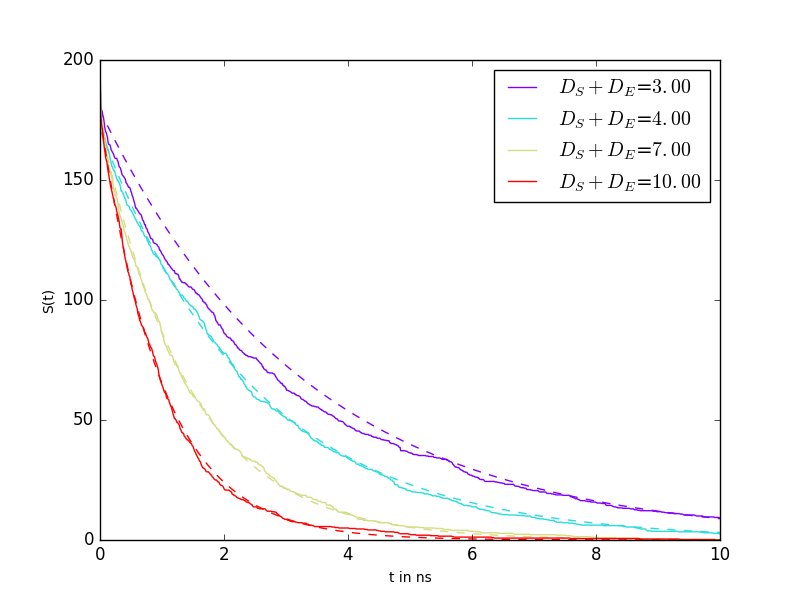
\includegraphics[width=\linewidth]{./data/besta.png}
  \captionsetup{width=0.9\linewidth}
  \captionof{figure}{Substrate particle number $S(t)$ for different Diffusion constants $D$ of the enzyme and substrate. With fitted theoretical curves from equation \cref{substratetheo}. The input parameters for RevReaDDy are: box size$=10^3nm$,reaction distance $=3$,intrinsic reaction rate$=10^{25}$, timesteps$=1000$,$S(0)=300$.}
  \label{fig:reactionssimulation}
\end{figure}
\newline \noindent In the second half of the master thesis fBm is going to be integrated in RevReaDDy. Similar simulations with fBm are going to be studied and related to Brownian motion. Spatial distributions of the reactants are going to be studied. The algorithm for fBm uses his velocity autocorrelation function. In principle it should be possible to integrate also different VACFs. The fBm integrator would result in an more general integrator, which could be used to model environments from real experiments. Including the VACF in the integrator may be an elegant way of adding an approximation due to the experimental environment. 

%\subsection{Code:Gebrochen-rationale Brownische Bewegung}
%\lstinputlisting[language=Python]{../simulation.py}

\nocite{}

%\printindex
\bibliography{literatur}
\bibliographystyle{plain}

\end{document}
